\documentclass[twoside,12pt]{mythesis}%this is the mythesis.cls file % twoside,openright,versioninfo
%\documentclass[12pt]{mythesis} %Change to single sided layout for softbound printing


% Consider:
% \newcommand{\ie}{i.\,e.}
% \newcommand{\Ie}{I.\,e.}
% \newcommand{\eg}{e.\,g.}
% \newcommand{\Eg}{E.\,g.}

\usepackage{fixltx2e}
\usepackage{textcomp}
\usepackage{fullpage}
\usepackage{float}
\usepackage{latexsym}
\usepackage{url}
\usepackage{epsfig}
\usepackage{graphicx}
\usepackage{amssymb}
\usepackage{amsmath}
\usepackage{bm}
\usepackage{array}
\usepackage[version=3]{mhchem}
\usepackage{ifthen}
\usepackage{caption}
\usepackage{hyperref}
\usepackage{amsthm}
\usepackage{amstext}
\usepackage{enumerate}
%\usepackage[osf]{mathpazo}
\usepackage{dcolumn}
\usepackage{lineno}
\usepackage{longtable}
\pagenumbering{arabic}

\newcolumntype{L}[1]{>{\raggedright\let\newline\\\arraybackslash\hspace{0pt}}m{#1}}
\newcolumntype{C}[1]{>{\centering\let\newline\\\arraybackslash\hspace{0pt}}m{#1}}
\newcolumntype{R}[1]{>{\raggedleft\let\newline\\\arraybackslash\hspace{0pt}}m{#1}}


\setcounter{tocdepth}{4}
\setcounter{secnumdepth}{4} %number of subsections that are allowed


%------------------------- 
%Add package to set page margins - probably only need this for the final printed version (two sided printing)?

\usepackage{geometry}

\geometry{
	a4paper,
	total={210mm,297mm},
	left={35mm},
    right={20mm},
	top={20mm},
	bottom={20mm},
}	
%Need to add it to the declaration and acknowledgements and list of figures
%--------------------------

%% Symbols
% unresolved:
\newcommand{\ud}{\mathrm{d}}
\newcommand{\drel}{\ensuremath{r_{\mathrm{rel}}}}
\newcommand{\nmax}{\ensuremath{n_\mathrm{max}}}

%Information for the title page
%Some of this is hard coded in mythesis.cls but you can over write if you need to
\title{Macroevolution with fossil and living taxa}

%
\author{Thomas Guillerme}
%
\month{\textsc{October}} \year{2015}
\previousdegrees{B.Sc., Universit\'{e}e Montpellier 2, 2010\\
                 M.Sc., Universit\'{e}e Montpellier 2, 2012}
\degreetitle{Doctor of Philosophy}
\institution{Trinity College Dublin}
\school{School of Natural Sciences}
\department{Zoology}

%End of preamble.
%--------------------------------------
\begin{document}

\maketitle %puts in your title

\chapter*{Declaration}
\addcontentsline{toc}{chapter}{Declaration}

I declare that this thesis has not been submitted as an exercise for a degree at this or any other University and it is, unless otherwise referenced, entirely my own work. I agree to deposit this thesis in the University's open access institutional repository or allow the library to do so on my behalf, subject to Irish Copyright Legislation and Trinity College Library conditions of use and acknowledgement.
\\
\\
\\

Thomas Guillerme
\chapter*{Summary}
\chaptermark{summary}
\addcontentsline{toc}{chapter}{Summary}

Hablbalbalbalbalba. Make it short!
% There is currently a problem with spacing somewhere so that Table of
% Contents, List of Tables, and List of Figures have the wrong amount
% of space.  Others are OK though...
\chapter*{Acknowledgements}
\addcontentsline{toc}{chapter}{Acknowledgements}

I would like to acknowledge Dr Rich FitzJohn for letting me use his thesis template!

%%% Local Variables:
%%% TeX-master: "thesis.tex"
%%% TeX-PDF-mode: t
%%% End:


%http://xkcd.com/1546/
%http://xkcd.com/722/

\allcontents %tells it to make a table of contents with figure and table lists too
 
\cleardoublepage
\mainbody

\chapter{Introduction}
\label{chap:introduction}

%Some quote from GG Simpson
%"Certainly paleontologists have found samples of an extremely small fraction, only, of the earth's extinct species, and even for groups that are most readily preserved and found as fossils they can never expect to find more than a fraction.""
%But I'm not sure, maybe not quote is better.


%---------------------
%
% GENERAL INTRO - MAKE IT SHORT
% 
%---------------------

% Why is all this important? Dig from Benton and Fritz et al
The amazing diversity of organisms living on the biosphere represents an overwhelmingly low fraction of the organisms that ever existed \citep{novacek1992ext,raup1993extinction}, yet, most of the work in biology focus solely on living species \citep{fritzdiversity2013}.
Ignoring this, can lead to misinterpretation of macroevolutionary or macroecological patterns \citep{jacksonwhat2006,quentaldiversity2010,dietlconservation2011,slaterunifying2013,fritzdiversity2013,benton2015}.


Although most species that have ever lived are now extinct \citep{novacek1992ext,raup1993extinction}, the majority of macroevolutionary studies focus solely on living species (e.g. \citealp{meredithimpacts2011,jetzthe2012})


% Natalie: Interspecific competition is the negative effect one species has upon another by consuming, or controlling access to, a resource that is limited in availability (Keddy 1989).

Studying events in the evolutionary history of a taxonomic group, such as adaptive radiation or extinction, requires a fine-­‐scale and accurate resolution of their phylogenetic relationships through time. To achieve this, most scientists would agree that information about both extant and extinct species is needed. However, few efforts have been made to combine extant and extinct species in the same phylogenetic trees; instead phylogenetic trees usually contain only extant species. Because the vast majority of species in a lineage will be represented by extinct species, studies focusing on extant species contain less than 0.1\% of the lineage’s species richness. In some clades, ignoring extinct species may also obscure the true evolutionary history, species richness (i.e. Proboscidea), biogeography (i.e. Tinamiforms) or ecological diversity (i.e. Crocodilomorphs). Thus including the fossil record in these kinds of studies is essential to fully understand the evolutionary history of lineages.

In some clades, ignoring extinct species may also obscure the true evolutionary history or diversity of a clade. For example, in mammals the orders Perissodactyla (horses, rhinos and tapirs) and Proboscidea (elephants and mammoths) currently contain only a few taxa although they contained many more species in the past (Cifelli 1981, Antoine et al. 2003, Mihlbachler 2008, Seiffert et al. 2012). Crocodilomorph reptiles also had much greater species diversity (there were ~45 genera during the Paleogene1 but only nine today - Martin 2009) and larger geographic ranges (e.g. extinct Crocodilomorpha remains are found in northern France - Hua 1997) in the past. Finally, ignoring extinct diversity can lead to misinterpretation in comparative phylogenetic studies. For example, ignoring extinct Dinornithiforms (Moas) leads to misinterpretation of both the diversification pattern and biogeography of ratites (Jetz et al. 2012). Thus including the fossil record in these kinds of studies is essential to fully understand the evolutionary history of lineages (Slater et al. 2012).

% Add crocs et al example from steering committees reports

%(Maybe add a figure showing the real evolutionary history (a tree  with data) and what we actually know of it (a tree with a lot of data at the top)

% Bits
% Although most species that have ever lived are now extinct \citep{novacek1992ext,raup1993extinction}, the many large-scale macroevolutionary studies focus solely on living species (e.g. \citealp{meredithimpacts2011,jetzthe2012}).
% Throughout history, life on Earth has suffered a series of mass extinction events resulting in drastic declines in global biodiversity \citep[e.g.][]{RaupPT,BentonPT,rennetime2013,Brusatte2015}.
% There is an increasing consensus among evolutionary biologists that studying both living and fossil taxa is essential for fully understanding macroevolutionary patterns and processes \cite{slaterunifying2013,fritzdiversity2013,Wood01032013}.

% Ignoring fossil taxa may lead to misinterpretation of macroevolutionary patterns and processes such as the timing of diversification events \citep[e.g.][]{pyrondivergence2011}, relationships among lineages \citep[e.g.][]{manosphylogeny2007} or niche occupancy \citep[e.g.][]{pearmanniche2008}.
% For example, including both living and fossil taxa in evolutionary studies can improve the accuracy of timing diversification events (e.g. \cite{ronquista2012}, our understanding of relationships among lineages (e.g. \cite{beckancient2014}, and our ability to infer biogeographical patterns through time (e.g. \cite{Meseguer01032015}.
% However, the long-term effects of mass extinctions are more varied \citep{Erwin1998344}, and include increases in species richness in some clades \citep{friedmanexplosive2010}, species richness declines in others \citep{Benton85}, changes in morphological diversity \citep{Ciampaglio2001,Ciampaglio2004,kornextinction2013} and shifts in ecological dominance \citep[e.g.][]{Brusatte12092008,toljagictriassic-jurassic2013,bensonfaunal2014}.

% This has led to increasing consensus among evolutionary biologists that fossil taxa should be included in macroevolutionary studies \citep{jacksonwhat2006,quentaldiversity2010,dietlconservation2011,slaterunifying2013,fritzdiversity2013}.
% To do this, however, we need to be able to place living and fossil taxa into the same phylogenies; a task that remains difficult despite recent methodological developments \citep[e.g.][]{pyrondivergence2011,ronquista2012,BEASTmaster}.
% To perform such analyses it is necessary to combine living and fossil taxa in phylogenetic trees.
% One increasingly popular method, the Total Evidence method \cite{eernissetaxonomic1993,ronquista2012}, combines molecular data from living taxa and morphological data from both living and fossil taxa in a supermatrix (e.g. \cite{pyrondivergence2011,ronquista2012,schragocombining2013,slaterunifying2013,beckancient2014,Meseguer01032015}, producing a phylogeny with living and fossil taxa at the tips. 
% These shifts are characterized by the decline of one clade that is replaced by a different unrelated clade with a similar ecological role (e.g. Brachiopoda and Bivalvia at the end Permian extinction \citealt{Sepkiski1981,CLAPHAM01102006} but see \citealt{Payne22052014}). 

% These phylogenies can be dated using methods such as tip-dating \cite{ronquista2012,Wood01032013} and incorporated into macroevolutionary studies (e.g. \cite{ronquista2012,Wood01032013,slaterphylogenetic2013}.
% Shifts in ecological dominance are of particular interest because they are a fairly common pattern observed in the fossil record (e.g. Foraminifera; \citealt{D'Hondt01011996,Coxall01042006}; Ichtyosauria; \citealt{thorneresetting2011}; Plesiosauria; \citealt{bensonfaunal2014}) and are often linked to major macroevolutionary processes such as adaptive \citep{Losos2010} or competitive radiations \citep{Brusatte12092008}.

\section{Combining data, methods and disciplines}

%§ 2 - How can we combine them
%How can we combine them. Traditional approach down up (morphology) but modern approach top down (molecules)
The traditional way to combine both living and fossils data is using morphological data for both and draw conclusions on want happened.
However the problem is that such approach simply exclude living species (e.g. trilobites) or use living species just as a way to branch the fossil species in a macroevolutionary context (e.g. O'Leary or any other big cladistic paper?).
Also, the methods use to describe relations can be have big artefacts (e.g. parsimony) or other approaches (Mk) model can be oversimplistic (but still usuable).
Finally the data for fossils is usually restricted to morphology and the few ecological traits that can be extract from that (e.g. diet from teeth but not behaviour or population size)
Another approach for looking at macroevolution is to solely use living species (e.g. Jetz) one can look at the differences between DNA (many differences, good) and use models that are more realistic than Mk because of only four states(e.g. GTR).
Also this method can include time by calibrating the molecular clocks using fossils (Zuckerkandl).
However, appart from the use of the fossils occurence dates for making the clock tick, this approach ignores all clades that have no living descendant (the majority of clades!) and can even poorlierly estimate things from fossils.

Therefore, combining both data allows use to palliate to some of the problems of both approaches!


%§ 3 - What can we do when we combine them?
%Interesting studies or examples?

%§ 4 - In this thesis I worked on both aspects: how to combine them (TEM + missing mammals) and what to do with them (STD)

\section{Phylogenies with living and fossil species}

TEM Intro on the data story.

\subsection{Chapter 2: Effects of missing data on topological inference using a Total Evidence approach}

%§ 5 -Introducing chapter 1
%TEM and missing data (link missing data)
In the first chapter, I run long term and thorough simulation to test how robust are our phylogenetic inferences when we combine living taxa with molecular and morphological to fossil taxa with morphological data only.
I particularly focused on how missing data in both living and fossil taxa can affect topology.
I found that the number of living taxa with available data is essential to recover accurate topologies.
Therefore we need data for living mammals, how much of it is out there?
(This chapter is currently in review in Molecular Phylogenetics and Evolution - revisions).

\subsection{Chapter 3: Morphological data availability in living mammals}
%§ 6 -%ntroducing chapter 2
%(link missing data) Missing data in mammals (link mammals)
Following these results, I was interested in showing practical implications of this effect and monitored the morphological data availability for living mammals.
I downloaded all the recent available morphological matrices and counted the number of living mammals with available morphological data.
I then tested how these taxa where distributed accross the phylogeny to check if there weren't clustered in some specific clades.
I found that a lot of data is missing but that at least most of it is randomly distributed and should not drastically effect topology.
So it's not so bad, but what can we do with these total evidence trees?
(This chapter is an invited submission to a special issue in Biology Letters. Submission is due in December 2015).

\section{Total evidence phylogenies applications}

Once we have these trees we can do loads of cool stuff (primates ideas).

\subsection{Chapter 4: Cretaceous-Palaeogene extinction does not affect mammalian disparity}

% Cheesy quote for that bit "The most erroneous stories are those we think we know best - and therefore never scrutinize or question." Gould whenever

%§ 7 -Introducing chapter 3
%(link mammals) STD with mammals (link to cool stuff)
One important step in explaining macroevolutionnary processes is to accurately describe the patterns.
For example, to explain the processes driving diversification or extinction during a mass extinction event, we need to accurately measure what's happening.
One classical example is the K-T extinction where the effects still remain unclear after so many years of research.
Because I showed in the previous chapters that mammals are ok for combinations, I studied how they get affected by K-T disparity wise (INTRODUCE DISPARITY FIRST).
I found that...
All the cool stuff we can do with TEM!
(This chapter will be submitted to Evolution).

\section{Further applications} % TG: I think if the title stays as shitty, no need for a title.

%§ 8 - Introducing discussion
%(link to cool stuff) end.
Finally I will discuss all these cool stuff and how research might develop by doing the combinations of data and looking at more accurate descriptors of patterns (e.g. diversity AND disparity) blalbalblabla.
%Add the bits of discussion from TEM new conclusion

%§ 9 - Additional work % TG: or that bit can go in the conclusion?
In addition I was also interested in a side project on developing tools for phylogenetic correction that takes into account tree uncertainty.
I participated to a collaborative project exploring drivers of longevity accross birds and mammals led by Kevin Healy.
I developed the implementation to take tree uncertainty into account and this is now an available R pckage (mulTree).
%In addition to that I also did longevity.
%I was involved in developing the method and running the analysis for this paper. Phylogenetic correction is one crucial aspect in accurately describing maco patterns. In the paper, along with the main author, we developed and implemented a method for allowing to include phylogenetic uncertainty in generalized linear mixed models.

\bibliography{References} 


%---------------------------------------------
%
%       START
%
%---------------------------------------------

\chapter[Missing data in living mammals]{Missing data in living mammals}
\label{chap:missing_mammals}

\bigskip
\medskip
\begin{center}

\noindent{\Large \bf Assessment of cladistic data availability for living mammals}
\footnote{A shorter version (2500 words) will be submitted under the same title to Biology Letters as an invited submission for a special issue on phylogenies with living and fossil species. This special issue is open to submission in December 2015. A pre-print is currently available as:
"Thomas Guillerme, Natalie Cooper. 2015. Assessment of cladistic data availability for living mammals. \textbf{bioRxiv}; doi: \href{http://dx.doi.org/10.1101/022970}{dx.doi.org/10.1101/022970}".}\footnote{\textit{Author contributions}: I designed the study, collected the data, ran the analyses and wrote the paper. NC helped design the study and commented on drafts of the manuscript.} \\

%} \\
% \medskip
% \noindent Key words: Total Evidence method, data structure, phylogenetic, fossil, topology\\
% \bigskip
% \noindent A shorter version (2500 words) will be submitted to Biology Letters as an invited submission for a special issue on phylogenies with living and fossil species. This special issue is open to submission in December 2015.\\

\end{center}
%---------------------------------------------
%
%       ABSTRACT
%
%---------------------------------------------


\section*{Abstract}
Analyses of living and fossil taxa are crucial for understanding changes in biodiversity through time.
The Total Evidence method allows living and fossil taxa to be combined in phylogenies, by using molecular data for living taxa and morphological data for both living and fossil taxa.
With this method, substantial overlap of morphological data among living and fossil taxa is crucial for accurately inferring topology.
However, although molecular data for living species is widely available, scientists using and generating morphological data mainly focus on fossils.
Therefore, there is a gap in our knowledge of neontological morphological data even in well-studied groups such as mammals.

We investigated the amount of morphological (cladistic) data available for living mammals and how this data was phylogenetically distributed across orders.
22 of 28 mammalian orders have \textless 25\% species with available morphological data; this has implications for the accurate placement of fossil taxa, although the issue is less pronounced at higher taxonomic levels. 
In most orders, species with available data are randomly distributed across the phylogeny, which may reduce the impact of the problem.
We suggest that increased morphological data collection efforts for living taxa are needed to produce accurate Total Evidence phylogenies. 


\newpage

%---------------------------------------------
%
%       INTRODUCTION
%
%---------------------------------------------
\newpage 
\section{Introduction}
There is an increasing consensus among evolutionary biologists that studying both living and fossil taxa is essential for fully understanding macroevolutionary patterns and processes \citep{slaterunifying2013,fritzdiversity2013,Wood01032013}.
For example, including both living and fossil taxa in evolutionary studies can improve the accuracy of timing diversification events \citep[e.g.][]{ronquista2012}, our understanding of relationships among lineages \citep[e.g.][]{beckancient2014}, and our ability to infer biogeographical patterns through time \citep[e.g.][]{Meseguer01032015}.
To perform such analyses it is necessary to combine living and fossil taxa in phylogenetic trees.
One increasingly popular method, the Total Evidence method \citep{eernissetaxonomic1993,ronquista2012}, combines molecular data from living taxa and morphological data from both living and fossil taxa in a supermatrix \citep[e.g.][]{pyrondivergence2011,ronquista2012,schragocombining2013,slaterunifying2013,beckancient2014,Meseguer01032015}, producing a phylogeny with living and fossil taxa at the tips. 
These phylogenies can be dated using methods such as tip-dating \citep{ronquista2012,Wood01032013} and incorporated into macroevolutionary studies \citep[e.g.][]{ronquista2012,Wood01032013,slaterphylogenetic2013}.

A downside of the Total Evidence method is that it requires a lot of data.
One must collect molecular data for living taxa and morphological data for both living and fossil taxa; two types of data that require fairly different technical skills (e.g. molecular sequencing \textit{vs.} anatomical description).
Additionally, large chunks of this data can be difficult, or even impossible, to collect for every taxon present in the analysis.
For example, fossils very rarely have molecular data and incomplete fossil preservation (e.g. soft \textit{vs.} hard tissues) may restrict the amount of morphological data available \citep{sansomfossilization2013}.
Additionally, since the molecular phylogenetics revolution, it has become less common to collect morphological characters for living taxa when molecular data are available (e.g. in \citep{slaterphylogenetic2013}, only 13\% of the 169 living taxa have coded morphological data).
Unfortunately this missing data can lead to errors in phylogenetic inference; in fact, simulations show that the ability of the Total Evidence method to recover the correct phylogenetic topology decreases when there is a low overlap between morphological data in the living and fossil taxa \citep{GuillermeCooper}, regardless the overall amount of morphological data available for the fossils (or the amount of molecular data available for the living species).
The effect of missing data on topology is greatest when living taxa have few morphological data.
This is because (1) a fossil cannot branch in the correct clade if there is no overlapping morphological data in the clade; and (2) a fossil has a higher probability of branching within a clade with more morphological data available for living taxa, regardless of whether this is the correct clade or not \citep{GuillermeCooper}. 

The issues above highlight that it is crucial to have sufficient morphological data for living taxa in a clade before using a Total Evidence approach.
However, it is unclear how much morphological data for living taxa is actually available (i.e. already coded from museum specimens and deposited in phylogenetic matrices accessible online), and how this data are distributed across clades.
Intuitively, most people assume this kind of data has already been collected, but empirical data suggest otherwise (e.g. in \citep{ronquista2012,slaterphylogenetic2013,beckancient2014}.
To investigate this further, we assess the amount of available morphological data for living mammals to determine whether sufficient data exists to build reliable Total Evidence phylogenies in this group.
We collected cladistic data (i.e. discrete morphological characters used in phylogenetics) from 286 phylogenetic matrices available online and measured the proportion of cladistic data available for each mammalian order.
%Additionally, if the available data are randomly distributed across clades, the topological errors should be less extreme than if the data are biased towards particulars groups.
Additionally, because missing morphological data in living species can influence tree topology as described above, %NC: Might still need to fix this sentence. "Topological caveats above" was too unclear.
we determined whether the available cladistic data was phylogenetically overdispersed or clustered in the mammalian orders where data was missing. 
We find that available morphological data for living mammals is scarce but generally randomly distributed across phylogenies. 
We recommend that efforts be made to collect and share more cladistic data for living species to improve the accuracy of Total Evidence phylogenies.

% NC: If there are word count problems we can ditch the last two sentences.
%---------------------------------------------
%
%       METHODS
%
%---------------------------------------------
\section{Materials and Methods}
\subsection{Data collection and standardisation}
We downloaded all cladistic matrices containing any living and/or fossil mammal taxa from three major public databases (accessed 10th of June 2015): Morphobank (\url{http://www.morphobank.org/}) \citep{morphobank}, Graeme Lloyd's website (\url{graemetlloyd.com/matrmamm.html}) and Ross Mounce's GitHub repository (\url{https://github.com/rossmounce/cladistic-data}).
We also performed a systematic Google Scholar search (accessed 11th of June 2015) for matrices that were not uploaded to these databases. We downloaded available matrices containing fossil and/or living mammal taxa from the three data bases using the following list of keywords:

\texttt{Mammalia; Monotremata; Marsupialia; Placentalia; Macroscelidea;\\
        Afrosoricida; Tubulidentata; Hyracoidea; Proboscidea; Sirenia; Pilosa;\\
        Cingulata; Scandentia; Dermoptera; Primates; Lagomorpha; Rodentia;\\
        Erinaceomorpha; Soricomorpha; Cetacea; Artiodactyla; Cetartiodactyla;\\
        Chiroptera; Perissodactyla; Pholidota; Carnivora; Didelphimorphia;\\
        Paucituberculata; Microbiotheria; Dasyuromorphia; Peramelemorphia;\\
        Notoryctemorphia; Diprotodontia}.

Note that some matrices have been downloaded from more than one database but that it is not an issue since we are interested in the total number of unique living OTUs and that if some where present in more than one matrix, they still only counted as one single OTU.

\subsubsection*{Morphobank}
We used the keywords listed above in the search menu of the Morphobank repository and downloaded the data associated with each project matching with the keywords.

\subsubsection*{Graeme Lloyd}
We downloaded all the matrices that were available with a direct download link in the mammal data section of Graeme Lloyd's website repository.

\subsubsection*{Ross Mounce}
We downloaded every 601 matrix from Ross Mounce's GitHub repository and then ran a shell script to select only the matrices that had any text element that match with one of the search terms.
To make the matrix selection more thorough, we ignored the keywords case as well as the latin suffix (\textit{ia}, \textit{ata}, \textit{ea}, and \textit{a}).

\subsubsection*{Google scholars}
To make sure we didn't miss any extra matrix that wasn't available on one of these repository, we ran a extra Google Scholar search. 
We downloaded the additional cladistic matrices from the 20 first search results matching with our selected keywords and with any of the 35 taxonomic levels (mammals Orders, Infraclasses and Class).
We used the following key words:

\texttt{\textit{order} ("morphology" OR "morphological" OR "cladistic") AND characters matrix paleontology phylogeny}

were \textit{order} was replaced by all the keywords listed above. For each 33 keywords, we selected the 20 first papers to match the Google search published since 2010 resulting in 660 papers.
Among these papers, not all contained relevant data (discrete morphological characters AND mammalian data).
We selected only the 20 first results per search term to avoid downloading articles that were to irrelevant. Among the 660 papers, only 50 contained a total of 425 extra living OTUs (Fig. ~\ref{Supp_figure_google_searches}).
Also we decided to select only the articles published since 2010 because nearly every one of the recent published matrix contains both a fraction of morphological characters and OTUs from previous studies.
For example in primates the character \textit{p7} coded first by \cite{ross1998phylogenetic} is reused with the same living species in \cite{seiffert2003fossil}, \cite{marivaux2005anthropoid}, \cite{seiffert2005basal}, \cite{bloch2007new}, \cite{bloch2007new}, \cite{kay2008anatomy}, \cite{silcox2008biogeographic}, \cite{seiffert2009convergent}, \cite{tabuce2009anthropoid}, \cite{boyer2010astragalar}, \cite{seiffert2010fossil}, \cite{marivaux2013djebelemur} and \cite{ni2013oldest}.

\begin{figure}[!h]
\centering
    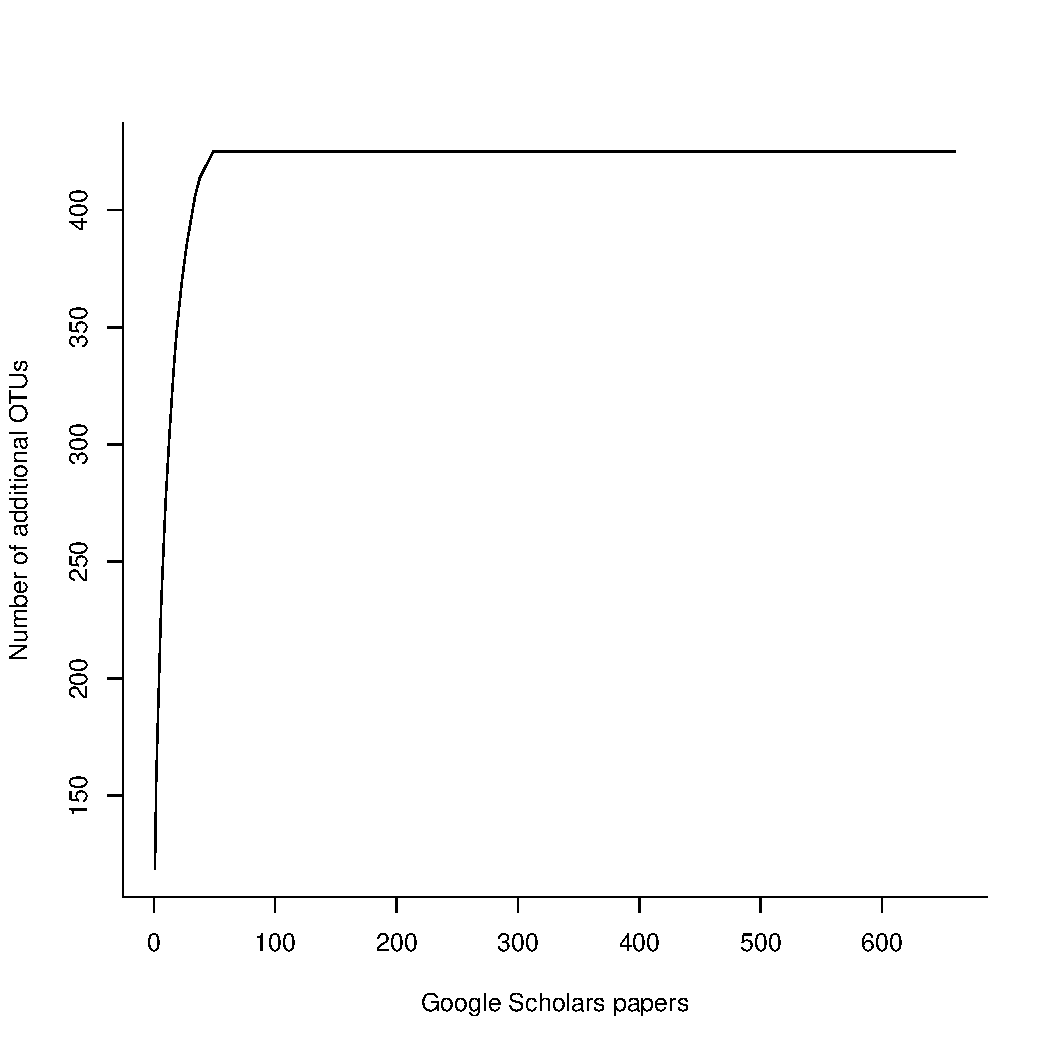
\includegraphics[width=1\textwidth]{Missing_mammals/Figures/Supp_figure_google_searches.pdf}
\caption[Google searches additional OTUs rarefaction curve.]{Google searches additional OTUs rarefaction curve. The x axis represent the number of google scholar matches (papers, books or abstracts) and the y axis represents the cumulative number of additional living OTUs per google scholar match.}
\label{Supp_figure_google_searches}
\end{figure}

We transformed all the non-nexus matrices (tnt, word, excel, jpeg) to nexus format manually.
In total, we downloaded 286 matrices containing a total of 11010 operational taxonomic units (OTUs) of which 5228 were unique.
In this study, we refer to OTUs rather than species since the entries in the downloaded matrices were not standardised and ranged from specific individual specimen names (i.e. the name of a collection item) to the family-level.
Where possible, we considered OTUs at their lowest valid taxonomic level (i.e. species) but some OTUs were only valid at a higher taxonomic level (e.g. genus or family).
Therefore for some orders, we sampled more genera than species (Table \ref{Table_results}).

To select the lowest valid taxonomic level for each OTU, we standardised their taxonomy by correcting species names so they matched standard taxonomic nomenclature (e.g., \textit{H. sapiens} was transformed to \textit{Homo sapiens}).
We designated as ``living'' all OTUs that were either present in the phylogeny of \citep{BinindaEmonds} or the taxonomy of \citep{wilson2005mammal}, and designated as ``fossil'' all OTUs that were present in the Paleobiology database (\url{https://paleobiodb.org/}).

For OTUs that did not appear in these three sources, we first decomposed the name (i.e. \textit{Homo sapiens} became \textit{Homo} and \textit{sapiens}) and tried to match the first element with a higher taxonomic level (genus or family).
Any OTUs that still had no matches in the sources above were designated as non-applicable (NA; see Fig. \ref{Supp_figure_Taxonomic_algorithm}).

\begin{figure}[!h]
\centering
    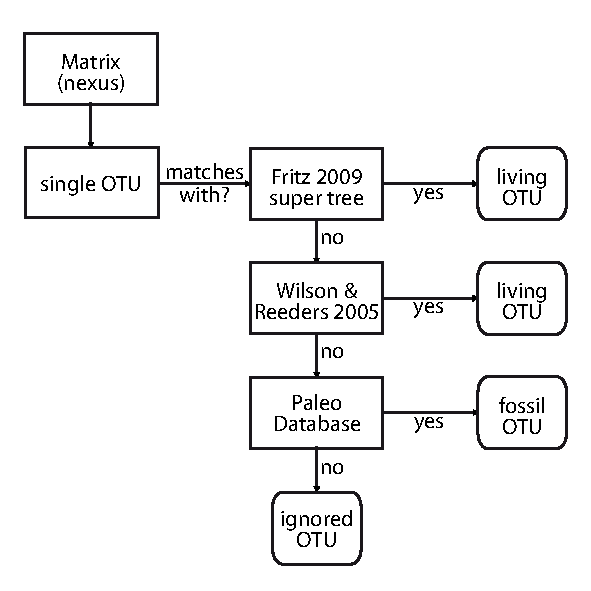
\includegraphics[width=1\textwidth]{Missing_mammals/Figures/Supp_figure_Taxonomic_algorithm.pdf}
\caption[Taxonomic matching algorithm used in this study.]{Taxonomic matching algorithm used in this study. For each matrix, each operational taxonomic units (OTU) is matched with the super tree from Bininda-Emonds 2007. If the OTU matches, then it is classified as living. Else it is matched with the Wilson \& Reeders 2005 taxonomy list. If the OTU matches, then it is classified as living. Else it is matched with the Paleo Database list of mammals. If the OTU matches, then it is classified as fossil. Else it is ignored.}
\label{Supp_figure_Taxonomic_algorithm}
\end{figure}

The number of characters in each matrix ranged from 6 to 4541.
Matrices with few characters are problematic when comparing available data among matrices because (1) they have less chance of having characters that overlap with those of other matrices \citep{wagner2000} and (2) they are more likely to contain a higher proportion of specific characters that are not-applicable across large clades \citep[e.g. ``antler ramifications'' is a character that is only applicable to Cervidae not all mammals][]{Brazeau2011}.
Therefore we selected only matrices containing \textgreater 100 characters for each OTU.
This threshold was chosen to correspond with the number of characters used in \citep{GuillermeCooper} and \citep{harrisonamong-character2014}.
Note that results of analyses with no character threshold are available in Supplementary Material. 
After removing all matrices with \textless 100 characters, we retained 1074 unique living mammal OTUs from 126 matrices for our analyses. % 1601 unique living OTUs for 286 matrices (no threshold)

\subsection{Data availability and distribution}
To assess the availability of cladistic data for each mammalian order, we calculated the percentage of OTUs with cladistic data at three different taxonomic levels: family, genus and species.
%We used these different taxonomic levels because some clades are well covered at the family- or genus-level, but poorly covered at the species-level. % NC: Probably obvious?
We consider orders with \textless 25\% of living taxa with cladistic data as having poor data coverage (``low'' coverage), and orders with \textgreater 75\% of living taxa with cladistic data as having good data coverage (hereafter ``high'' coverage). 

For orders with \textless 100\% cladistic data coverage at any taxonomic level, we investigated whether the available cladistic data was (i) randomly distributed, (ii) overdispersed or (iii) clustered, with respect to phylogeny, using two metrics from community phylogenetics: the Nearest Taxon Index (NTI; \citep{webb2002phylogenies} and the Net Relatedness Index (NRI; \citep{webb2002phylogenies}. 
NTI is most sensitive to clustering or overdispersion near the tips, whereas NRI is more sensitive to clustering or overdispersion across the whole phylogeny \citep{Cooper2008}. 
Both metrics were calculated using the \texttt{picante} package in R \citep{picante,R}.

NTI \citep{webb2002phylogenies} is based on mean nearest neighbour distance (MNND) and is calculated as follows:
  \begin{equation}
    NTI=-\left(\frac{\overline{MNND}_{obs}-\overline{MNND}_{n}}{\sigma(MNND_{n})}\right)
  \end{equation}
where $\overline{MNND}_{obs}$ is the observed mean distance between each of $n$ taxa with cladistic data and its nearest neighbour with cladistic data in the phylogeny, 
$\overline{MNND}_{n}$ is the mean of 1000 mean MNND between $n$ randomly drawn taxa, and $\sigma(MNND_{n})$ is the standard deviation of these 1000 random MNND values.
NRI is similar but is based on mean phylogenetic distance (MPD) as follows:
  \begin{equation}
    NRI=-\left(\frac{\overline{MPD}_{obs}-\overline{MPD}_{n}}{\sigma(MPD_{n})}\right)
  \end{equation}
where $\overline{MPD}_{obs}$ is the observed mean phylogenetic distance of the tree containing only the $n$ taxa with cladistic data, $\overline{MPD}_{n}$ is the expected random MPD for $n$ taxa estimated by calculating the MPD from $n$ taxa randomly drawn from the phylogeny and repeated 1000 times, and $\sigma(MPD_{n})$ is the standard deviation of the 1000 random MPD values. % NC: This can be shortened a bit but it's only gonna save you 50 words max.
Negative NTI and NRI values show that the focal taxa are more overdispersed across the phylogeny than expected by chance, and positive values reflect significant clustering.

We calculated NTI and NRI values for each mammalian order separately, at each different taxonomic level. 
For each analysis our focal taxa were those with available cladistic data at that taxonomic level and the phylogeny was the phylogeny of the order pruned from \citep{BinindaEmonds}.

%---------------------------------------------
%
%       RESULTS
%
%---------------------------------------------

\section{Results}
Across the 126 cladistic matrices we extracted, 22 out of 28 mammalian orders have low coverage (\textless 25\% of species with cladistic data) and six have high coverage (\textgreater 75\% of species with cladistic data) at the species-level.
At the genus-level, three orders have low coverage and 12 have high coverage, and at the family-level, no orders have low coverage and 23 have high coverage (Table \ref{Table_results}).

% latex table generated in R 3.2.0 by xtable 1.7-4 package
% Sun Jun 21 15:26:40 2015
\begin{longtable}{lL{1.8cm}C{2cm}lcc}
\caption{Number of taxa with available cladistic data for mammalian orders at three taxonomic levels. The left vertical bar represents ``low'' coverage (\textless 25\%); the right vertical bar represents ``high'' coverage (\textgreater 75\%). A negative Net Relatedness Index (NRI) and Nearest Taxon Index (NTI) shows more phylogeneticaly dispersed taxa than expected by chance; a positive value shows more phylogeneticaly clustered taxa than expected by chance. Significant NRI or NTI values are highlighted in bold. One star (*) signifies a p-value between 0.05 and 0.005; two starts between 0.005 and 0.0005 and three stars \textless 0.0005.} \\ 
  \hline
Order & Taxonomic level & Proportion of taxa & Coverage & NRI & NTI \\ 
  \hline
Afrosoricida & family & 2/2 & 
\includegraphics[width=0.20\linewidth, height=0.05\linewidth]{Missing_mammals/Table_figures/bar1.pdf} &   &   \\ 
  Afrosoricida & genus & 17/17 & 
\includegraphics[width=0.20\linewidth, height=0.05\linewidth]{Missing_mammals/Table_figures/bar2.pdf} &   &   \\ 
  \textbf{Afrosoricida} & \textbf{species} & \textbf{23/42} & 
\includegraphics[width=0.20\linewidth, height=0.05\linewidth]{Missing_mammals/Table_figures/bar3.pdf} & \textbf{1.89*} & 1.19 \\ 
  Carnivora & family & 11/15 & 
\includegraphics[width=0.20\linewidth, height=0.05\linewidth]{Missing_mammals/Table_figures/bar4.pdf} & 0.43 & 1.68 \\ 
  \textbf{Carnivora} & \textbf{genus} & \textbf{30/125} & 
\includegraphics[width=0.20\linewidth, height=0.05\linewidth]{Missing_mammals/Table_figures/bar5.pdf} & \textbf{4.14**} & \textbf{1.81*} \\ 
  \textbf{Carnivora} & \textbf{species} & \textbf{42/283} & 
\includegraphics[width=0.20\linewidth, height=0.05\linewidth]{Missing_mammals/Table_figures/bar6.pdf} & \textbf{18.64**} & \textbf{3.02**} \\ 
  Cetartiodactyla & family & 21/21 & 
\includegraphics[width=0.20\linewidth, height=0.05\linewidth]{Missing_mammals/Table_figures/bar7.pdf} &   &   \\ 
  \textbf{Cetartiodactyla} & \textbf{genus} & \textbf{77/128} & 
\includegraphics[width=0.20\linewidth, height=0.05\linewidth]{Missing_mammals/Table_figures/bar8.pdf} & 0.87 & \textbf{1.77*} \\ 
  \textbf{Cetartiodactyla} & \textbf{species} & \textbf{129/310} & 
\includegraphics[width=0.20\linewidth, height=0.05\linewidth]{Missing_mammals/Table_figures/bar9.pdf} & \textbf{2.72*} & 0.04 \\ 
  Chiroptera & family & 13/18 & 
\includegraphics[width=0.20\linewidth, height=0.05\linewidth]{Missing_mammals/Table_figures/bar10.pdf} & 0.55 & 0.63 \\ 
  \textbf{Chiroptera} & \textbf{genus} & \textbf{85/202} & 
\includegraphics[width=0.20\linewidth, height=0.05\linewidth]{Missing_mammals/Table_figures/bar11.pdf} & \textbf{16.91**} & \textbf{2.85**} \\ 
  \textbf{Chiroptera} & \textbf{species} & \textbf{165/1053} & 
\includegraphics[width=0.20\linewidth, height=0.05\linewidth]{Missing_mammals/Table_figures/bar12.pdf} & \textbf{14.55**} & \textbf{3.44**} \\ 
  Cingulata & family & 1/1 & 
\includegraphics[width=0.20\linewidth, height=0.05\linewidth]{Missing_mammals/Table_figures/bar13.pdf} &   &   \\ 
  Cingulata & genus & 8/9 & 
\includegraphics[width=0.20\linewidth, height=0.05\linewidth]{Missing_mammals/Table_figures/bar14.pdf} & 1.49 & -1.63 \\ 
  Cingulata & species & 6/29 & 
\includegraphics[width=0.20\linewidth, height=0.05\linewidth]{Missing_mammals/Table_figures/bar15.pdf} & 1.43 & 0.36 \\ 
  Dasyuromorphia & family & 2/2 & 
\includegraphics[width=0.20\linewidth, height=0.05\linewidth]{Missing_mammals/Table_figures/bar16.pdf} &   &   \\ 
  Dasyuromorphia & genus & 7/22 & 
\includegraphics[width=0.20\linewidth, height=0.05\linewidth]{Missing_mammals/Table_figures/bar17.pdf} & -1 & -1.45 \\ 
  Dasyuromorphia & species & 8/64 & 
\includegraphics[width=0.20\linewidth, height=0.05\linewidth]{Missing_mammals/Table_figures/bar18.pdf} & -1.15 & -0.62 \\ 
  Dermoptera & family & 1/1 & 
\includegraphics[width=0.20\linewidth, height=0.05\linewidth]{Missing_mammals/Table_figures/bar19.pdf} &   &   \\ 
  Dermoptera & genus & 1/2 & 
\includegraphics[width=0.20\linewidth, height=0.05\linewidth]{Missing_mammals/Table_figures/bar20.pdf} &   &   \\ 
  Dermoptera & species & 1/2 & 
\includegraphics[width=0.20\linewidth, height=0.05\linewidth]{Missing_mammals/Table_figures/bar21.pdf} &   &   \\ 
  Didelphimorphia & family & 1/1 & 
\includegraphics[width=0.20\linewidth, height=0.05\linewidth]{Missing_mammals/Table_figures/bar22.pdf} &   &   \\ 
  Didelphimorphia & genus & 16/16 & 
\includegraphics[width=0.20\linewidth, height=0.05\linewidth]{Missing_mammals/Table_figures/bar23.pdf} &   &   \\ 
  Didelphimorphia & species & 40/84 & 
\includegraphics[width=0.20\linewidth, height=0.05\linewidth]{Missing_mammals/Table_figures/bar24.pdf} & -0.94 & 0.36 \\ 
  Diprotodontia & family & 9/11 & 
\includegraphics[width=0.20\linewidth, height=0.05\linewidth]{Missing_mammals/Table_figures/bar25.pdf} & -0.8 & 0.56 \\ 
  Diprotodontia & genus & 20/38 & 
\includegraphics[width=0.20\linewidth, height=0.05\linewidth]{Missing_mammals/Table_figures/bar26.pdf} & -1.36 & -0.73 \\ 
  Diprotodontia & species & 16/126 & 
\includegraphics[width=0.20\linewidth, height=0.05\linewidth]{Missing_mammals/Table_figures/bar27.pdf} & -2.29 & -1.55 \\ 
  Erinaceomorpha & family & 1/1 & 
\includegraphics[width=0.20\linewidth, height=0.05\linewidth]{Missing_mammals/Table_figures/bar28.pdf} &   &   \\ 
  Erinaceomorpha & genus & 10/10 & 
\includegraphics[width=0.20\linewidth, height=0.05\linewidth]{Missing_mammals/Table_figures/bar29.pdf} &   &   \\ 
  Erinaceomorpha & species & 21/22 & 
\includegraphics[width=0.20\linewidth, height=0.05\linewidth]{Missing_mammals/Table_figures/bar30.pdf} & -1.1 & -0.3 \\ 
  Hyracoidea & family & 1/1 & 
\includegraphics[width=0.20\linewidth, height=0.05\linewidth]{Missing_mammals/Table_figures/bar31.pdf} &   &   \\ 
  Hyracoidea & genus & 1/3 & 
\includegraphics[width=0.20\linewidth, height=0.05\linewidth]{Missing_mammals/Table_figures/bar32.pdf} &   &   \\ 
  Hyracoidea & species & 1/4 & 
\includegraphics[width=0.20\linewidth, height=0.05\linewidth]{Missing_mammals/Table_figures/bar33.pdf} &   &   \\ 
  Lagomorpha & family & 1/2 & 
\includegraphics[width=0.20\linewidth, height=0.05\linewidth]{Missing_mammals/Table_figures/bar34.pdf} &   &   \\ 
  Lagomorpha & genus & 1/12 & 
\includegraphics[width=0.20\linewidth, height=0.05\linewidth]{Missing_mammals/Table_figures/bar35.pdf} &   &   \\ 
  Lagomorpha & species & 1/86 & 
\includegraphics[width=0.20\linewidth, height=0.05\linewidth]{Missing_mammals/Table_figures/bar36.pdf} &   &   \\ 
  Macroscelidea & family & 1/1 & 
\includegraphics[width=0.20\linewidth, height=0.05\linewidth]{Missing_mammals/Table_figures/bar37.pdf} &   &   \\ 
  Macroscelidea & genus & 4/4 & 
\includegraphics[width=0.20\linewidth, height=0.05\linewidth]{Missing_mammals/Table_figures/bar38.pdf} &   &   \\ 
  Macroscelidea & species & 5/15 & 
\includegraphics[width=0.20\linewidth, height=0.05\linewidth]{Missing_mammals/Table_figures/bar39.pdf} & -0.98 & -1.38 \\ 
  Microbiotheria & family & 1/1 & 
\includegraphics[width=0.20\linewidth, height=0.05\linewidth]{Missing_mammals/Table_figures/bar40.pdf} &   &   \\ 
  Microbiotheria & genus & 1/1 & 
\includegraphics[width=0.20\linewidth, height=0.05\linewidth]{Missing_mammals/Table_figures/bar41.pdf} &   &   \\ 
  Microbiotheria & species & 1/1 & 
\includegraphics[width=0.20\linewidth, height=0.05\linewidth]{Missing_mammals/Table_figures/bar42.pdf} &   &   \\ 
  Monotremata & family & 2/2 & 
\includegraphics[width=0.20\linewidth, height=0.05\linewidth]{Missing_mammals/Table_figures/bar43.pdf} &   &   \\ 
  Monotremata & genus & 2/3 & 
\includegraphics[width=0.20\linewidth, height=0.05\linewidth]{Missing_mammals/Table_figures/bar44.pdf} & -0.71 & -0.71 \\ 
  Monotremata & species & 2/4 & 
\includegraphics[width=0.20\linewidth, height=0.05\linewidth]{Missing_mammals/Table_figures/bar45.pdf} & -1.01 & -1.03 \\ 
  Notoryctemorphia & family & 1/1 & 
\includegraphics[width=0.20\linewidth, height=0.05\linewidth]{Missing_mammals/Table_figures/bar46.pdf} &   &   \\ 
  Notoryctemorphia & genus & 1/1 & 
\includegraphics[width=0.20\linewidth, height=0.05\linewidth]{Missing_mammals/Table_figures/bar47.pdf} &   &   \\ 
  Notoryctemorphia & species & 0/2 & 
\includegraphics[width=0.20\linewidth, height=0.05\linewidth]{Missing_mammals/Table_figures/bar48.pdf} &   &   \\ 
  Paucituberculata & family & 1/1 & \includegraphics[width=0.20\linewidth, height=0.05\linewidth]{Missing_mammals/Table_figures/bar49.pdf} &   &   \\ 
  Paucituberculata & genus & 2/3 & \includegraphics[width=0.20\linewidth, height=0.05\linewidth]{Missing_mammals/Table_figures/bar50.pdf} & 0 & 0 \\ 
  Paucituberculata & species & 2/5 & \includegraphics[width=0.20\linewidth, height=0.05\linewidth]{Missing_mammals/Table_figures/bar51.pdf} & -0.64 & -0.65 \\ 
  Peramelemorphia & family & 2/2 & \includegraphics[width=0.20\linewidth, height=0.05\linewidth]{Missing_mammals/Table_figures/bar52.pdf} &   &   \\ 
  Peramelemorphia & genus & 7/7 & \includegraphics[width=0.20\linewidth, height=0.05\linewidth]{Missing_mammals/Table_figures/bar53.pdf} &   &   \\ 
  Peramelemorphia & species & 16/18 & \includegraphics[width=0.20\linewidth, height=0.05\linewidth]{Missing_mammals/Table_figures/bar54.pdf} & -0.09 & 1 \\ 
  Perissodactyla & family & 3/3 & \includegraphics[width=0.20\linewidth, height=0.05\linewidth]{Missing_mammals/Table_figures/bar55.pdf} &   &   \\ 
  Perissodactyla & genus & 6/6 & \includegraphics[width=0.20\linewidth, height=0.05\linewidth]{Missing_mammals/Table_figures/bar56.pdf} &   &   \\ 
  Perissodactyla & species & 7/16 & \includegraphics[width=0.20\linewidth, height=0.05\linewidth]{Missing_mammals/Table_figures/bar57.pdf} & 0.62 & -2.5 \\ 
  Pholidota & family & 1/1 & \includegraphics[width=0.20\linewidth, height=0.05\linewidth]{Missing_mammals/Table_figures/bar58.pdf} &   &   \\ 
  Pholidota & genus & 1/1 & \includegraphics[width=0.20\linewidth, height=0.05\linewidth]{Missing_mammals/Table_figures/bar59.pdf} &   &   \\ 
  \textbf{Pholidota} & \textbf{species} & \textbf{3/8} & \includegraphics[width=0.20\linewidth, height=0.05\linewidth]{Missing_mammals/Table_figures/bar60.pdf} & \textbf{2.64*} & \textbf{2.23*} \\ 
  Pilosa & family & 3/5 & \includegraphics[width=0.20\linewidth, height=0.05\linewidth]{Missing_mammals/Table_figures/bar61.pdf} & 0.94 & 0.93 \\ 
  Pilosa & genus & 3/5 & \includegraphics[width=0.20\linewidth, height=0.05\linewidth]{Missing_mammals/Table_figures/bar62.pdf} & -0.36 & -0.31 \\ 
  Pilosa & species & 3/29 & \includegraphics[width=0.20\linewidth, height=0.05\linewidth]{Missing_mammals/Table_figures/bar63.pdf} & 0.33 & 0.79 \\ 
  Primates & family & 15/15 & \includegraphics[width=0.20\linewidth, height=0.05\linewidth]{Missing_mammals/Table_figures/bar64.pdf} &   &   \\ 
  Primates & genus & 48/68 & \includegraphics[width=0.20\linewidth, height=0.05\linewidth]{Missing_mammals/Table_figures/bar65.pdf} & -0.41 & -1.4 \\ 
  Primates & species & 56/351 & \includegraphics[width=0.20\linewidth, height=0.05\linewidth]{Missing_mammals/Table_figures/bar66.pdf} & -1.6 & -2.04 \\ 
  Proboscidea & family & 1/1 & \includegraphics[width=0.20\linewidth, height=0.05\linewidth]{Missing_mammals/Table_figures/bar67.pdf} &   &   \\ 
  Proboscidea & genus & 1/2 & \includegraphics[width=0.20\linewidth, height=0.05\linewidth]{Missing_mammals/Table_figures/bar68.pdf} &   &   \\ 
  Proboscidea & species & 1/3 & \includegraphics[width=0.20\linewidth, height=0.05\linewidth]{Missing_mammals/Table_figures/bar69.pdf} &   &   \\ 
  Rodentia & family & 11/32 & \includegraphics[width=0.20\linewidth, height=0.05\linewidth]{Missing_mammals/Table_figures/bar70.pdf} & -0.46 & -1.91 \\ 
  Rodentia & genus & 21/450 & \includegraphics[width=0.20\linewidth, height=0.05\linewidth]{Missing_mammals/Table_figures/bar71.pdf} & -2.11 & 0.3 \\ 
  Rodentia & species & 15/2094 & \includegraphics[width=0.20\linewidth, height=0.05\linewidth]{Missing_mammals/Table_figures/bar72.pdf} & -1.65 & -2.55 \\ 
  Scandentia & family & 2/2 & \includegraphics[width=0.20\linewidth, height=0.05\linewidth]{Missing_mammals/Table_figures/bar73.pdf} &   &   \\ 
  Scandentia & genus & 2/5 & \includegraphics[width=0.20\linewidth, height=0.05\linewidth]{Missing_mammals/Table_figures/bar74.pdf} & -0.77 & -0.76 \\ 
  Scandentia & species & 2/20 & \includegraphics[width=0.20\linewidth, height=0.05\linewidth]{Missing_mammals/Table_figures/bar75.pdf} & -1.79 & -1.99 \\ 
  Sirenia & family & 2/2 & \includegraphics[width=0.20\linewidth, height=0.05\linewidth]{Missing_mammals/Table_figures/bar76.pdf} &   &   \\ 
  Sirenia & genus & 2/2 & \includegraphics[width=0.20\linewidth, height=0.05\linewidth]{Missing_mammals/Table_figures/bar77.pdf} &   &   \\ 
  Sirenia & species & 4/4 & \includegraphics[width=0.20\linewidth, height=0.05\linewidth]{Missing_mammals/Table_figures/bar78.pdf} &   &   \\ 
  Soricomorpha & family & 3/4 & \includegraphics[width=0.20\linewidth, height=0.05\linewidth]{Missing_mammals/Table_figures/bar79.pdf} & -0.93 & -0.92 \\ 
  \textbf{Soricomorpha} & \textbf{genus} & \textbf{19/43} & \includegraphics[width=0.20\linewidth, height=0.05\linewidth]{Missing_mammals/Table_figures/bar80.pdf} & \textbf{6.98**} & \textbf{2.49*} \\ 
  \textbf{Soricomorpha} & \textbf{species} & \textbf{19/392} & \includegraphics[width=0.20\linewidth, height=0.05\linewidth]{Missing_mammals/Table_figures/bar81.pdf} & \textbf{13.19**} & \textbf{3.89**} \\ 
  Tubulidentata & family & 1/1 & \includegraphics[width=0.20\linewidth, height=0.05\linewidth]{Missing_mammals/Table_figures/bar82.pdf} &   &   \\ 
  Tubulidentata & genus & 1/1 & \includegraphics[width=0.20\linewidth, height=0.05\linewidth]{Missing_mammals/Table_figures/bar83.pdf} &   &   \\ 
  Tubulidentata & species & 1/1 & \includegraphics[width=0.20\linewidth, height=0.05\linewidth]{Missing_mammals/Table_figures/bar84.pdf} &   &   \\ 
   \hline
\hline
\label{Table_results}
\end{longtable}


Among the mammalian orders containing OTUs with no available cladistic data, only six orders had significantly clustered data (Carnivora, Cetartiodactyla, Chiroptera and Soricomorpha at both species- and genus-level and Afrosoricida and Pholidota at the species-level only) and no order had significantly overdispersed data at any taxonomic level (Table \ref{Table_results}).

Two contrasting results are shown in Fig. \ref{Figure_example_coverage} with randomly distributed OTUs with cladistic data in Primates (Fig. \ref{Figure_example_coverage}A) and phylogenetically clustered OTUs with cladistic data in Carnivora (mainly Canidae; Fig. \ref{Figure_example_coverage}B).

\begin{figure}[!h]
\centering
    \includegraphics[width=1\textwidth]{Missing_mammals/Figures/example_coverage.pdf}
\caption[Phylogenetic distribution of species with available cladistic data across Primates and Carnivora]{Phylogenetic distribution of species with available cladistic data across two mammalian orders (A: Primates; B: Carnivora).
Edges are colored in grey when no cladistic data are available for a species and in blue when data are available.}
\label{Figure_example_coverage}
\end{figure}

%---------------------------------------------
%
%       DISCUSSION
%
%---------------------------------------------

\section{Discussion}
Our results show that although phylogenetic relationships among living mammals are well-resolved \citep[e.g.][]{BinindaEmonds,meredithimpacts2011} , most of the data used to build these phylogenies is molecular, and very little cladistic data are available for living mammals compared to fossil mammals \citep[e.g.][]{O'Leary08022013,ni2013oldest}.
This has implications for building Total Evidence phylogenies containing both living and fossil mammals, as without sufficient cladistic data for living species, fossil placements in these trees are very uncertain \citep{GuillermeCooper}.
Cladistic data coverage in living mammals varies across taxonomic levels and in its phylogenetic distribution.
Higher taxonomic levels are always better sampled than lower ones and within these taxonomic levels, the available data are mostly randomly distributed across the phylogeny, apart from in six orders).

The number of living mammalian taxa with no available cladistic data was surprisingly high at the species-level: only six out of 28 orders have a high coverage of taxa with available cladistic data (and two of the 28 orders are monospecific!).
This high coverage threshold of 75\% of taxa with available cladistic data represents the minimum amount of data required before missing data has a significant effect on the topology of Total Evidence trees \citep{GuillermeCooper}.
Beyond this threshold, there is considerable displacement of wildcard taxa \citep[\textit{sensu}][]{kearneyfragmentary2002} and decreases in clade conservation \citep{GuillermeCooper}.
Therefore we expect a high probability of topological artefacts for the placement of fossil taxa at the species-level in most mammalian orders.
However, data coverage seems to be less of an issue at higher taxonomic levels (i.e. genus- and family-level).
This point is important from a practical point of view because of the slight discrepancy between the neontological and palaeontological concept of species.
While neontological species are described using morphology, genetic distance, spatial distribution and even behaviour, palaeontological species can be based only on morphological, spatial and temporal data \citep[e.g.][]{ni2013oldest}.
Because of this, most palaeontological studies are using the genus as their smallest OTU \citep[e.g.][]{ni2013oldest,O'Leary08022013}.
Thus data availability at the genus-level in living mammals should be our primary concern when aiming to build phylogenies of living and fossil taxa.

When only a few species with cladistic data are available, the ideal scenario is for them to be phylogenetically overdispersed (i.e. that there is data for at least every sub-clade) to maximize the possibilities of a fossil branching from the right clade.
The second best scenario is that species with cladistic data are randomly distributed across the phylogeny. 
In this scenario we expect no special bias in the placement of the fossil \citep{GuillermeCooper}, it is therefore encouraging that for most orders, species with cladistic data were randomly distributed across the phylogeny of each order.
The worst case scenario for fossil placement is that species with cladistic data are phylogenetically clustered. 
In this situation we expect two major biases to occur: first, the fossil will not be able to branch within a clade containing no data, and second, the fossil will have a higher probability, at random, of branching within the clade containing most of the available data.
This means that fossils with uncertain phylogenetic affinities (\textit{incertae sedis} will have a higher probability of branching within the most sampled clade just by chance).
Our results suggest that this may be an issue, at the genus-level, in Carnivora, Cetartiodactyla, Chiroptera and Soricomorpha. 
For example, a Carnivora fossil will be unable to branch in the Herpestidae that has no species with cladistic data, and will also have more chance to branch, randomly, within the Canidae clade than any other clade in Carnivora (Fig. \ref{Figure_example_coverage}B).
Thus, in Total Evidence trees, placements of some carnivoran fossils should considered with caution. 
% NC: Trying not to piss off GraHam - really it's weird stuff appearing in Carnivora that we are concerned by, not all Carnivora. TG: I think it's mainly Graham's work that focuses on canids.
In this study, we treated all cladistic matrices as equal in a similar way to molecular matrices. 
For example, if matrix A contained 100 characters for taxa X and Y, and matrix B contained 50 different characters for taxa X and Z, we assumed that both matrices can be combined in a supermatrix containing 150 independent characters for taxon X, 100 for taxon Y and 50 for taxon Z.
Unfortunately, cladistic data cannot always be treated in this way because some characters may overlap.
For example, if matrix A has a character coding for the shape of a particular morphological feature and matrix B has a character coding for the presence of this same morphological feature and a second character coding for its shape, then these three characters are non-independent compound characters \citep{Brazeau2011}.
However, in reasonably sized matrices \citep[\textgreater 100 characters;][]{GuillermeCooper,harrisonamong-character2014} it is more likely that a number of characters are consistently conserved among the different matrices and thus easily combinable.
For example, within the Primate cladistic literature, the character \textit{p7} - the size of the $4^{th}$ lower premolar paraconid - has been used consistently for \textgreater 15 years \citep[e.g.][]{ross1998phylogenetic,marivaux2005anthropoid,ni2013oldest} and can therefore be combined among the matrices.
A conservative approach to avoid compound characters would be to select only the most recent matrix for each group, but this would result in the loss of a lot of data.

Despite the absence of good cladistic data coverage for living mammals, the Total Evidence methods still seems to be the most promising way of combining living and fossil data for macroevolutionary analyses. 
Following the recommendations in \citep{GuillermeCooper}, we need to code cladistic characters for as many living species possible. 
Fortunately, data for living mammals is usually readily available in natural history collections, therefore, we propose that an increased effort be put into coding morphological characters from living species, possibly by engaging in collaborative data collection projects through web portals such as \textit{MorphoBank} \citep{morphobank}.
% NC: Still feels like it needs one final sentence to round it all off. Many something like below, but less crappy:
Such an effort would be valuable not only to phylogeneticists, but also to any researcher focusing understanding macroevolutionary patterns and processes.%interested in the diversity of life on Earth.

%Biology letters various stuff

% \bibliographystyle{sysbio}
% \bibliography{References}

%\section{SOM}
%\newcommand{\beginsupplement}{%
%    \setcounter{table}{0}
%    \renewcommand{\thetable}{S\arabic{table}}%
%    \setcounter{figure}{0}
%    \renewcommand{\thefigure}{S\arabic{figure}}%
%}
%\beginsupplement
%
\noindent{\Large \bf Supplementary Material}

\begin{figure}[!htbp]
\centering
    \includegraphics[width=1\textwidth]{Missing_mammals/Supplementary/MissingDataFigure.pdf}
\caption{Example of topological errors due to missing morphological data in living taxa.
The phylogeny contains two clades, Aves and Mammalia, with molecular data (grey) for both but only morphological data (red) for Aves.
If a mammalian fossil species (with no molecular data) is added to the phylogeny, it will erroneously branch with the Aves instead of the Mammalia because no morphological data will overlap between the fossil mammals and the living ones.}
\label{Figure_missing_data_problem}
\end{figure}

\bigskip

\section{Data collection}
1- Data collection: key words, clade (ordinal) metacharacters, Google Search terms, Google Search protocol, Google Search rarefaction curve.

\subsection{Public repositories}
We downloaded available matrices containing fossil and/or living mammal taxa from the three following data bases using the following list of keywords:

\texttt{Mammalia; Monotremata; Marsupialia; Placentalia; Macroscelidea; Afrosoricida; Tubulidentata; Hyracoidea; Proboscidea; Sirenia; Pilosa; Cingulata; Scandentia; Dermoptera; Primates; Lagomorpha; Rodentia; Erinaceomorpha; Soricomorpha; Cetacea; Artiodactyla; Cetartiodactyla; Chiroptera; Perissodactyla; Pholidota; Carnivora; Didelphimorphia; Paucituberculata; Microbiotheria; Dasyuromorphia; Peramelemorphia; Notoryctemorphia; Diprotodontia}.

Details about each public repository specific search option is listed below. Note that some matrices have been downloaded from more than one database but that it is not an issue since we are interested in the total number of living OTUs and that if some where present in more than one matrix, they still only counted as a unique OTU.

\subsubsection{Morphobank}
We accessed the Morphobank repository (\texttt{http://www.morphobank.org/}) on the 5th of December 2014 and used the keywords listed above in the search menue. We downloaded the data associated with each project matching with the keyword.

\subsubsection{Graeme Lloyd}
We accessed Graeme Lloyd's website repository (\texttt{http://graemetlloyd.com/}) on the 5th of December 2014 and downloaded all the matrices that were available with a direct download link in the mammal data section of the website (\texttt{http://graemetlloyd.com/matrmamm.html}).

\subsubsection{Ross Mounce}
We accessed Ross Mounce's GitHub repository (\texttt{https://github.com/rossmounce}) on the 2nd of December 2014 and downloaded every 601 matrix. We then ran a shell script to select only the matrices that had any text element that match with one of the search terms. To make the matrix selection more thorough, we ignored the keywords case as well as the latin suffix (\textit{ia}, \textit{ata}, \textit{ea}, and \textit{a}).

\subsection{Google scholars}
To make sure we didn't miss any extra matrix that wasn't available on one of these repository, we ran a Google Scholar search on the 5th of January. 
We downloaded the additional cladistic matrices from the 20 first search results matching with our selected keywords and with any of the 35 taxonomic levels (mammals Orders, Infraclasses and Class).
We used the following key words:

\texttt{\textit{order} ("morphology" OR "morphological" OR "cladistic") AND characters matrix paleontology phylogeny}

were \textit{order} was replaced by all the keywords listed above. For each 33 keywords, we selected the 20 first papers to match the Google search published since 2010 resulting in 660 papers. Among these papers, not all contained relevant data (discrete morphological characters AND mammalian data). We selected only the 20 first results per search term to avoid downloading articles that were to irrelevant. Among the 660 papers, only 50 contained a total of 425 extra living OTUs (figure ~\ref{Supp_figure_google_searches}).
Also we decided to select only the articles published since 2010 because nearly every one of the recent published matrix contains both a fraction of morphological characters and OTUs from previous studies. For example in primates the character \textit{p7} coded first by \cite{ross1998phylogenetic} is reused with the same living species in \cite{seiffert2003fossil}, \cite{marivaux2005anthropoid}, \cite{seiffert2005basal}, \cite{bloch2007new}, \cite{bloch2007new}, \cite{kay2008anatomy}, \cite{silcox2008biogeographic}, \cite{seiffert2009convergent}, \cite{tabuce2009anthropoid}, \cite{boyer2010astragalar}, \cite{seiffert2010fossil}, \cite{marivaux2013djebelemur} and \cite{ni2013oldest}.

\begin{figure}[!htbp]
\centering
    \includegraphics[width=1\textwidth]{Missing_mammals/Supplementary/Supp_figure_google_searches.pdf}
\caption{Google searches additional OTUs rarefaction curve. The x axis represent the number of google scholar matches (papers, books or abstracts) and the y axis represents the cumulative number of additional living OTUs per google scholar match.}
\label{Supp_figure_google_searches}
\end{figure}

\subsection{Standardising the matrices}
We transformed all the non-nexus matrices (tnt, word, excel, jpeg) to nexus format manually. We then cleaned the nexus matrices by removing any extra information (trees, continuous characters, morphological characters description, molecular data) to end up with nexus matrices containing only the discrete morphological data. We then manually fixed the wrong bionomial names format (e.g. \textit{H. sapiens}) into the correct ones (e.g. \textit{Homo sapiens}) using the abbreviation list in the concerned publications. 

\subsection{Selecting the living OTUs}
Finally we applied a taxonomic matching algorithm to classify the OTUs as either living or fossil. The algorithm is matching every OTU name from every matrix with one of the following taxonomic references: the list of taxa from the Fritz \textit{et al.} supertree (2009) \cite{FritzTree}; the taxonomic list from the Wilson and Reeder's Mammals Species of the World (2005) \cite{wilson2005mammal} and the list of all the mammal fossil from the Paleobio Database (\texttt{http://paleobiodb.org/cgi-bin/bridge.pl?a=login}) accessed on the 13th of Janurary 2015. The OTUs that matched with one of the two first references were considered as living OTUs, the OTUs matching with the third reference were considered as fossil OTUs, finally, the OTUs matching with non of the references were discarded (figure ~\ref{Supp_figure_Taxonomic_algorithm}).

\begin{figure}[!htbp]
\centering
    \includegraphics[width=1\textwidth]{Missing_mammals/Supplementary/Supp_figure_Taxonomic_algorithm.pdf}
\caption{Taxonomic matching algorithm used in this study. For each matrix, each operational taxonomic units (OTU) is matched with the super tree from Fritz 2009. If the OTU matches, then it is classified as living. Else it is matched with the Wilson \& Reeders 2005 taxonomy list. If the OTU matches, then it is classified as living. Else it is matched with the Paleo Database list of mammals. If the OTU matches, then it is classified as fossil. Else it is ignored.}
\label{Supp_figure_Taxonomic_algorithm}
\end{figure}

%\bibliographystyle{vancouver}
%\bibliography{Supp_References}

\section{Supplementary results}
The following section contains supplementary results to the main body: the available data structure using the NTI and the PD metric; the proportion of available data and the data structure for all the matrices (including the matrices with less than 100 characters); and phylogenetical representation of the data availability per order (excluding Primates and Carnivora, present in the main body).

% latex table generated in R 3.2.0 by xtable 1.7-4 package
% Sat Jun 20 17:19:07 2015
\begin{longtable}{lL{1.8cm}C{2cm}lcc}
\caption{Number of taxa with available cladistic data for mammalian orders at three taxonomic levels (without any character threshold; results from the 286 matrices). The coverage represents the proportion of taxa with available morphological data. The left vertical bar represents 25\% of available data (``low'' coverage if \textless 25\%); The right vertical bar represents 75\% of available data (``high'' coverage if \textgreater 75\%). When the Net Relatedness Index (NRI) and the Nearest Taxon Index (NTI) are negative, taxa are more phylogenetically dispersed than expected by chance; when NRI or NTI are positive, taxa are more phylogenetically clustered by expected by chance. Significant NRI or NTI are highlighted in bold. One star (*) represents a p-value between 0.05 and 0.005; two starts between 0.005 and 0.0005 and three stars a p-value less than 0.0005.} \\ 
  \hline
Order & Taxonomic level & Proportion of taxa & Coverage & NRI & NTI \\ 
  \hline
Afrosoricida & family & 2/2 & \includegraphics[width=0.20\linewidth, height=0.05\linewidth]{Missing_mammals/Supplementary/Results_1c/Table_figures/bar1.pdf} &   &   \\ 
  Afrosoricida & genus & 17/17 & \includegraphics[width=0.20\linewidth, height=0.05\linewidth]{Missing_mammals/Supplementary/Results_1c/Table_figures/bar2.pdf} &   &   \\ 
  Afrosoricida & species & 23/42 & \includegraphics[width=0.20\linewidth, height=0.05\linewidth]{Missing_mammals/Supplementary/Results_1c/Table_figures/bar3.pdf} & 1.75 & 1.08 \\ 
  Carnivora & family & 14/15 & \includegraphics[width=0.20\linewidth, height=0.05\linewidth]{Missing_mammals/Supplementary/Results_1c/Table_figures/bar4.pdf} & 0.63 & 0.6 \\ 
  \textbf{Carnivora} & \textbf{genus} & \textbf{54/125} & \includegraphics[width=0.20\linewidth, height=0.05\linewidth]{Missing_mammals/Supplementary/Results_1c/Table_figures/bar5.pdf} & \textbf{4.81**} & \textbf{1.78*} \\ 
  \textbf{Carnivora} & \textbf{species} & \textbf{76/283} & \includegraphics[width=0.20\linewidth, height=0.05\linewidth]{Missing_mammals/Supplementary/Results_1c/Table_figures/bar6.pdf} & \textbf{7.66**} & \textbf{0.85} \\ 
  Cetartiodactyla & family & 21/21 & \includegraphics[width=0.20\linewidth, height=0.05\linewidth]{Missing_mammals/Supplementary/Results_1c/Table_figures/bar7.pdf} &   &   \\ 
  Cetartiodactyla & genus & 100/128 & \includegraphics[width=0.20\linewidth, height=0.05\linewidth]{Missing_mammals/Supplementary/Results_1c/Table_figures/bar8.pdf} & 0.85 & 0.94 \\ 
  \textbf{Cetartiodactyla} & \textbf{species} & \textbf{171/310} & \includegraphics[width=0.20\linewidth, height=0.05\linewidth]{Missing_mammals/Supplementary/Results_1c/Table_figures/bar9.pdf} & \textbf{1.92*} & \textbf{-0.46} \\ 
  Chiroptera & family & 15/18 & \includegraphics[width=0.20\linewidth, height=0.05\linewidth]{Missing_mammals/Supplementary/Results_1c/Table_figures/bar10.pdf} & -0.28 & 0.56 \\ 
  \textbf{Chiroptera} & \textbf{genus} & \textbf{93/202} & \includegraphics[width=0.20\linewidth, height=0.05\linewidth]{Missing_mammals/Supplementary/Results_1c/Table_figures/bar11.pdf} & \textbf{13.47**} & \textbf{1.1} \\ 
  \textbf{Chiroptera} & \textbf{species} & \textbf{215/1053} & \includegraphics[width=0.20\linewidth, height=0.05\linewidth]{Missing_mammals/Supplementary/Results_1c/Table_figures/bar12.pdf} & \textbf{8.82**} & \textbf{1.22} \\ 
  Cingulata & family & 1/1 & \includegraphics[width=0.20\linewidth, height=0.05\linewidth]{Missing_mammals/Supplementary/Results_1c/Table_figures/bar13.pdf} &   &   \\ 
  Cingulata & genus & 8/9 & \includegraphics[width=0.20\linewidth, height=0.05\linewidth]{Missing_mammals/Supplementary/Results_1c/Table_figures/bar14.pdf} & 1.51 & -1.57 \\ 
  \textbf{Cingulata} & \textbf{species} & \textbf{9/29} & \includegraphics[width=0.20\linewidth, height=0.05\linewidth]{Missing_mammals/Supplementary/Results_1c/Table_figures/bar15.pdf} & \textbf{1.9*} & \textbf{0.11} \\ 
  Dasyuromorphia & family & 2/2 & \includegraphics[width=0.20\linewidth, height=0.05\linewidth]{Missing_mammals/Supplementary/Results_1c/Table_figures/bar16.pdf} &   &   \\ 
  Dasyuromorphia & genus & 8/22 & \includegraphics[width=0.20\linewidth, height=0.05\linewidth]{Missing_mammals/Supplementary/Results_1c/Table_figures/bar17.pdf} & -0.75 & -1.07 \\ 
  Dasyuromorphia & species & 9/64 & \includegraphics[width=0.20\linewidth, height=0.05\linewidth]{Missing_mammals/Supplementary/Results_1c/Table_figures/bar18.pdf} & -0.88 & -0.34 \\ 
  Dermoptera & family & 1/1 & \includegraphics[width=0.20\linewidth, height=0.05\linewidth]{Missing_mammals/Supplementary/Results_1c/Table_figures/bar19.pdf} &   &   \\ 
  Dermoptera & genus & 1/2 & \includegraphics[width=0.20\linewidth, height=0.05\linewidth]{Missing_mammals/Supplementary/Results_1c/Table_figures/bar20.pdf} &   &   \\ 
  Dermoptera & species & 1/2 & \includegraphics[width=0.20\linewidth, height=0.05\linewidth]{Missing_mammals/Supplementary/Results_1c/Table_figures/bar21.pdf} &   &   \\ 
  Didelphimorphia & family & 1/1 & \includegraphics[width=0.20\linewidth, height=0.05\linewidth]{Missing_mammals/Supplementary/Results_1c/Table_figures/bar22.pdf} &   &   \\ 
  Didelphimorphia & genus & 16/16 & \includegraphics[width=0.20\linewidth, height=0.05\linewidth]{Missing_mammals/Supplementary/Results_1c/Table_figures/bar23.pdf} &   &   \\ 
  Didelphimorphia & species & 42/84 & \includegraphics[width=0.20\linewidth, height=0.05\linewidth]{Missing_mammals/Supplementary/Results_1c/Table_figures/bar24.pdf} & -1.65 & 0.2 \\ 
  Diprotodontia & family & 11/11 & \includegraphics[width=0.20\linewidth, height=0.05\linewidth]{Missing_mammals/Supplementary/Results_1c/Table_figures/bar25.pdf} &   &   \\ 
  Diprotodontia & genus & 25/38 & \includegraphics[width=0.20\linewidth, height=0.05\linewidth]{Missing_mammals/Supplementary/Results_1c/Table_figures/bar26.pdf} & -1.13 & -1.31 \\ 
  Diprotodontia & species & 31/126 & \includegraphics[width=0.20\linewidth, height=0.05\linewidth]{Missing_mammals/Supplementary/Results_1c/Table_figures/bar27.pdf} & 0.48 & -1.77 \\ 
  Erinaceomorpha & family & 1/1 & \includegraphics[width=0.20\linewidth, height=0.05\linewidth]{Missing_mammals/Supplementary/Results_1c/Table_figures/bar28.pdf} &   &   \\ 
  Erinaceomorpha & genus & 10/10 & \includegraphics[width=0.20\linewidth, height=0.05\linewidth]{Missing_mammals/Supplementary/Results_1c/Table_figures/bar29.pdf} &   &   \\ 
  Erinaceomorpha & species & 21/22 & \includegraphics[width=0.20\linewidth, height=0.05\linewidth]{Missing_mammals/Supplementary/Results_1c/Table_figures/bar30.pdf} & -1.07 & -0.2 \\ 
  Hyracoidea & family & 1/1 & \includegraphics[width=0.20\linewidth, height=0.05\linewidth]{Missing_mammals/Supplementary/Results_1c/Table_figures/bar31.pdf} &   &   \\ 
  Hyracoidea & genus & 1/3 & \includegraphics[width=0.20\linewidth, height=0.05\linewidth]{Missing_mammals/Supplementary/Results_1c/Table_figures/bar32.pdf} &   &   \\ 
  Hyracoidea & species & 1/4 & \includegraphics[width=0.20\linewidth, height=0.05\linewidth]{Missing_mammals/Supplementary/Results_1c/Table_figures/bar33.pdf} &   &   \\ 
  Lagomorpha & family & 2/2 & \includegraphics[width=0.20\linewidth, height=0.05\linewidth]{Missing_mammals/Supplementary/Results_1c/Table_figures/bar34.pdf} &   &   \\ 
  Lagomorpha & genus & 5/12 & \includegraphics[width=0.20\linewidth, height=0.05\linewidth]{Missing_mammals/Supplementary/Results_1c/Table_figures/bar35.pdf} & -1.06 & -0.95 \\ 
  Lagomorpha & species & 12/86 & \includegraphics[width=0.20\linewidth, height=0.05\linewidth]{Missing_mammals/Supplementary/Results_1c/Table_figures/bar36.pdf} & -0.62 & -1.88 \\ 
  Macroscelidea & family & 1/1 & \includegraphics[width=0.20\linewidth, height=0.05\linewidth]{Missing_mammals/Supplementary/Results_1c/Table_figures/bar37.pdf} &   &   \\ 
  Macroscelidea & genus & 4/4 & \includegraphics[width=0.20\linewidth, height=0.05\linewidth]{Missing_mammals/Supplementary/Results_1c/Table_figures/bar38.pdf} &   &   \\ 
  Macroscelidea & species & 12/15 & \includegraphics[width=0.20\linewidth, height=0.05\linewidth]{Missing_mammals/Supplementary/Results_1c/Table_figures/bar39.pdf} & -1.3 & -1.06 \\ 
  Microbiotheria & family & 1/1 & \includegraphics[width=0.20\linewidth, height=0.05\linewidth]{Missing_mammals/Supplementary/Results_1c/Table_figures/bar40.pdf} &   &   \\ 
  Microbiotheria & genus & 1/1 & \includegraphics[width=0.20\linewidth, height=0.05\linewidth]{Missing_mammals/Supplementary/Results_1c/Table_figures/bar41.pdf} &   &   \\ 
  Microbiotheria & species & 1/1 & \includegraphics[width=0.20\linewidth, height=0.05\linewidth]{Missing_mammals/Supplementary/Results_1c/Table_figures/bar42.pdf} &   &   \\ 
  Monotremata & family & 2/2 & \includegraphics[width=0.20\linewidth, height=0.05\linewidth]{Missing_mammals/Supplementary/Results_1c/Table_figures/bar43.pdf} &   &   \\ 
  Monotremata & genus & 2/3 & \includegraphics[width=0.20\linewidth, height=0.05\linewidth]{Missing_mammals/Supplementary/Results_1c/Table_figures/bar44.pdf} & -0.72 & -0.69 \\ 
  Monotremata & species & 2/4 & \includegraphics[width=0.20\linewidth, height=0.05\linewidth]{Missing_mammals/Supplementary/Results_1c/Table_figures/bar45.pdf} & -0.97 & -0.97 \\ 
  Notoryctemorphia & family & 1/1 & \includegraphics[width=0.20\linewidth, height=0.05\linewidth]{Missing_mammals/Supplementary/Results_1c/Table_figures/bar46.pdf} &   &   \\ 
  Notoryctemorphia & genus & 1/1 & \includegraphics[width=0.20\linewidth, height=0.05\linewidth]{Missing_mammals/Supplementary/Results_1c/Table_figures/bar47.pdf} &   &   \\ 
  Notoryctemorphia & species & 0/2 & \includegraphics[width=0.20\linewidth, height=0.05\linewidth]{Missing_mammals/Supplementary/Results_1c/Table_figures/bar48.pdf} &   &   \\ 
  Paucituberculata & family & 1/1 & \includegraphics[width=0.20\linewidth, height=0.05\linewidth]{Missing_mammals/Supplementary/Results_1c/Table_figures/bar49.pdf} &   &   \\ 
  Paucituberculata & genus & 3/3 & \includegraphics[width=0.20\linewidth, height=0.05\linewidth]{Missing_mammals/Supplementary/Results_1c/Table_figures/bar50.pdf} &   &   \\ 
  Paucituberculata & species & 5/5 & \includegraphics[width=0.20\linewidth, height=0.05\linewidth]{Missing_mammals/Supplementary/Results_1c/Table_figures/bar51.pdf} &   &   \\ 
  Peramelemorphia & family & 2/2 & \includegraphics[width=0.20\linewidth, height=0.05\linewidth]{Missing_mammals/Supplementary/Results_1c/Table_figures/bar52.pdf} &   &   \\ 
  Peramelemorphia & genus & 7/7 & \includegraphics[width=0.20\linewidth, height=0.05\linewidth]{Missing_mammals/Supplementary/Results_1c/Table_figures/bar53.pdf} &   &   \\ 
  Peramelemorphia & species & 16/18 & \includegraphics[width=0.20\linewidth, height=0.05\linewidth]{Missing_mammals/Supplementary/Results_1c/Table_figures/bar54.pdf} & -0.13 & 0.97 \\ 
  Perissodactyla & family & 3/3 & \includegraphics[width=0.20\linewidth, height=0.05\linewidth]{Missing_mammals/Supplementary/Results_1c/Table_figures/bar55.pdf} &   &   \\ 
  Perissodactyla & genus & 6/6 & \includegraphics[width=0.20\linewidth, height=0.05\linewidth]{Missing_mammals/Supplementary/Results_1c/Table_figures/bar56.pdf} &   &   \\ 
  Perissodactyla & species & 10/16 & \includegraphics[width=0.20\linewidth, height=0.05\linewidth]{Missing_mammals/Supplementary/Results_1c/Table_figures/bar57.pdf} & -0.07 & -2.63 \\ 
  Pholidota & family & 1/1 & \includegraphics[width=0.20\linewidth, height=0.05\linewidth]{Missing_mammals/Supplementary/Results_1c/Table_figures/bar58.pdf} &   &   \\ 
  Pholidota & genus & 1/1 & \includegraphics[width=0.20\linewidth, height=0.05\linewidth]{Missing_mammals/Supplementary/Results_1c/Table_figures/bar59.pdf} &   &   \\ 
  Pholidota & species & 4/8 & \includegraphics[width=0.20\linewidth, height=0.05\linewidth]{Missing_mammals/Supplementary/Results_1c/Table_figures/bar60.pdf} & 1.18 & 0.94 \\ 
  Pilosa & family & 4/5 & \includegraphics[width=0.20\linewidth, height=0.05\linewidth]{Missing_mammals/Supplementary/Results_1c/Table_figures/bar61.pdf} & 1.87 & 2 \\ 
  Pilosa & genus & 4/5 & \includegraphics[width=0.20\linewidth, height=0.05\linewidth]{Missing_mammals/Supplementary/Results_1c/Table_figures/bar62.pdf} & -0.96 & 0.36 \\ 
  \textbf{Pilosa} & \textbf{species} & \textbf{5/29} & \includegraphics[width=0.20\linewidth, height=0.05\linewidth]{Missing_mammals/Supplementary/Results_1c/Table_figures/bar63.pdf} & \textbf{1.28} & \textbf{2.38*} \\ 
  Primates & family & 15/15 & \includegraphics[width=0.20\linewidth, height=0.05\linewidth]{Missing_mammals/Supplementary/Results_1c/Table_figures/bar64.pdf} &   &   \\ 
  Primates & genus & 48/68 & \includegraphics[width=0.20\linewidth, height=0.05\linewidth]{Missing_mammals/Supplementary/Results_1c/Table_figures/bar65.pdf} & -0.35 & -1.33 \\ 
  Primates & species & 64/351 & \includegraphics[width=0.20\linewidth, height=0.05\linewidth]{Missing_mammals/Supplementary/Results_1c/Table_figures/bar66.pdf} & -0.67 & -1.27 \\ 
  Proboscidea & family & 1/1 & \includegraphics[width=0.20\linewidth, height=0.05\linewidth]{Missing_mammals/Supplementary/Results_1c/Table_figures/bar67.pdf} &   &   \\ 
  Proboscidea & genus & 2/2 & \includegraphics[width=0.20\linewidth, height=0.05\linewidth]{Missing_mammals/Supplementary/Results_1c/Table_figures/bar68.pdf} &   &   \\ 
  Proboscidea & species & 2/3 & \includegraphics[width=0.20\linewidth, height=0.05\linewidth]{Missing_mammals/Supplementary/Results_1c/Table_figures/bar69.pdf} & -0.69 & -0.69 \\ 
  Rodentia & family & 18/32 & \includegraphics[width=0.20\linewidth, height=0.05\linewidth]{Missing_mammals/Supplementary/Results_1c/Table_figures/bar70.pdf} & 0.66 & -0.98 \\ 
  Rodentia & genus & 82/450 & \includegraphics[width=0.20\linewidth, height=0.05\linewidth]{Missing_mammals/Supplementary/Results_1c/Table_figures/bar71.pdf} & -1.66 & 1.55 \\ 
  \textbf{Rodentia} & \textbf{species} & \textbf{90/2094} & \includegraphics[width=0.20\linewidth, height=0.05\linewidth]{Missing_mammals/Supplementary/Results_1c/Table_figures/bar72.pdf} & \textbf{2.76*} & \textbf{2.34*} \\ 
  Scandentia & family & 2/2 & \includegraphics[width=0.20\linewidth, height=0.05\linewidth]{Missing_mammals/Supplementary/Results_1c/Table_figures/bar73.pdf} &   &   \\ 
  Scandentia & genus & 2/5 & \includegraphics[width=0.20\linewidth, height=0.05\linewidth]{Missing_mammals/Supplementary/Results_1c/Table_figures/bar74.pdf} & -0.74 & -0.74 \\ 
  Scandentia & species & 3/20 & \includegraphics[width=0.20\linewidth, height=0.05\linewidth]{Missing_mammals/Supplementary/Results_1c/Table_figures/bar75.pdf} & -1.88 & -0.84 \\ 
  Sirenia & family & 2/2 & \includegraphics[width=0.20\linewidth, height=0.05\linewidth]{Missing_mammals/Supplementary/Results_1c/Table_figures/bar76.pdf} &   &   \\ 
  Sirenia & genus & 2/2 & \includegraphics[width=0.20\linewidth, height=0.05\linewidth]{Missing_mammals/Supplementary/Results_1c/Table_figures/bar77.pdf} &   &   \\ 
  Sirenia & species & 4/4 & \includegraphics[width=0.20\linewidth, height=0.05\linewidth]{Missing_mammals/Supplementary/Results_1c/Table_figures/bar78.pdf} &   &   \\ 
  Soricomorpha & family & 3/4 & \includegraphics[width=0.20\linewidth, height=0.05\linewidth]{Missing_mammals/Supplementary/Results_1c/Table_figures/bar79.pdf} & -0.98 & -0.99 \\ 
  \textbf{Soricomorpha} & \textbf{genus} & \textbf{19/43} & \includegraphics[width=0.20\linewidth, height=0.05\linewidth]{Missing_mammals/Supplementary/Results_1c/Table_figures/bar80.pdf} & \textbf{7.11**} & \textbf{2.59**} \\ 
  \textbf{Soricomorpha} & \textbf{species} & \textbf{21/392} & \includegraphics[width=0.20\linewidth, height=0.05\linewidth]{Missing_mammals/Supplementary/Results_1c/Table_figures/bar81.pdf} & \textbf{10.65**} & \textbf{3.56**} \\ 
  Tubulidentata & family & 1/1 & \includegraphics[width=0.20\linewidth, height=0.05\linewidth]{Missing_mammals/Supplementary/Results_1c/Table_figures/bar82.pdf} &   &   \\ 
  Tubulidentata & genus & 1/1 & \includegraphics[width=0.20\linewidth, height=0.05\linewidth]{Missing_mammals/Supplementary/Results_1c/Table_figures/bar83.pdf} &   &   \\ 
  Tubulidentata & species & 1/1 & \includegraphics[width=0.20\linewidth, height=0.05\linewidth]{Missing_mammals/Supplementary/Results_1c/Table_figures/bar84.pdf} &   &   \\ 
   \hline
\hline
\label{Table_results}
\end{longtable}


\begin{figure}[!htbp]
\centering
    \includegraphics[width=1\textwidth]{Missing_mammals/Supplementary/Supp_figure_AFROSORICIDA.pdf}
\caption{Distribution of available morphological data across Afrosoricida. Edges are colored in grey when no morphological data is available or in blue when data is available.}
\label{Supp_Figure_Phylo-Afrosoricida}
\end{figure}

\begin{figure}[!htbp]
\centering
    \includegraphics[width=1\textwidth]{Missing_mammals/Supplementary/Supp_figure_CHIROPTERA.pdf}
\caption{Distribution of available morphological data across Chiroptera. Edges are colored in grey when no morphological data is available or in blue when data is available.}
\label{Supp_Figure_Phylo-Chiroptera}
\end{figure}

\begin{figure}[!htbp]
\centering
    \includegraphics[width=1\textwidth]{Missing_mammals/Supplementary/Supp_figure_CINGULATA.pdf}
\caption{Distribution of available morphological data across Cingulata. Edges are colored in grey when no morphological data is available or in blue when data is available.}
\label{Supp_Figure_Phylo-Cingulata}
\end{figure}

\begin{figure}[!htbp]
\centering
    \includegraphics[width=1\textwidth]{Missing_mammals/Supplementary/Supp_figure_DASYUROMORPHIA.pdf}
\caption{Distribution of available morphological data across Dasyuromorphia. Edges are colored in grey when no morphological data is available or in blue when data is available.}
\label{Supp_Figure_Phylo-Dasyuromorphia}
\end{figure}

\begin{figure}[!htbp]
\centering
    \includegraphics[width=1\textwidth]{Missing_mammals/Supplementary/Supp_figure_DIDELPHIMORPHIA.pdf}
\caption{Distribution of available morphological data across Didelphimorphia. Edges are colored in grey when no morphological data is available or in blue when data is available.}
\label{Supp_Figure_Phylo-Didelphimorphia}
\end{figure}

\begin{figure}[!htbp]
\centering
    \includegraphics[width=1\textwidth]{Missing_mammals/Supplementary/Supp_figure_DIPROTODONTIA.pdf}
\caption{Distribution of available morphological data across Diprotodontia. Edges are colored in grey when no morphological data is available or in blue when data is available.}
\label{Supp_Figure_Phylo-Diprotodontia}
\end{figure}

\begin{figure}[!htbp]
\centering
    \includegraphics[width=1\textwidth]{Missing_mammals/Supplementary/Supp_figure_ERINACEOMORPHA.pdf}
\caption{Distribution of available morphological data across Erinaceomorpha. Edges are colored in grey when no morphological data is available or in blue when data is available.}
\label{Supp_Figure_Phylo-Erinaceomorpha}
\end{figure}

\begin{figure}[!htbp]
\centering
    \includegraphics[width=1\textwidth]{Missing_mammals/Supplementary/Supp_figure_PILOSA.pdf}
\caption{Distribution of available morphological data across Pilosa. Edges are colored in grey when no morphological data is available or in blue when data is available.}
\label{Supp_Figure_Phylo-Pilosa}
\end{figure}

\begin{figure}[!htbp]
\centering
    \includegraphics[width=1\textwidth]{Missing_mammals/Supplementary/Supp_figure_CETARTIODACTYLA.pdf}
\caption{Distribution of available morphological data across Cetartiodactyla. Edges are colored in grey when no morphological data is available or in blue when data is available.}
\label{Supp_Figure_Phylo-Primates}
\end{figure}

\begin{figure}[!htbp]
\centering
    \includegraphics[width=1\textwidth]{Missing_mammals/Supplementary/Supp_figure_RODENTIA.pdf}
\caption{Distribution of available morphological data across Rodentia. Edges are colored in grey when no morphological data is available or in blue when data is available.}
\label{Supp_Figure_Phylo-Rodentia}
\end{figure}

\begin{figure}[!htbp]
\centering
    \includegraphics[width=1\textwidth]{Missing_mammals/Supplementary/Supp_figure_SCANDENTIA.pdf}
\caption{Distribution of available morphological data across Scandentia. Edges are colored in grey when no morphological data is available or in blue when data is available.}
\label{Supp_Figure_Phylo-Scandentia}
\end{figure}

\begin{figure}[!htbp]
\centering
    \includegraphics[width=1\textwidth]{Missing_mammals/Supplementary/Supp_figure_SORICOMORPHA.pdf}
\caption{Distribution of available morphological data across Soricomorpha. Edges are colored in grey when no morphological data is available or in blue when data is available.}
\label{Supp_Figure_Phylo-Soricomorpha}
\end{figure}


%END
%\end{document}
	
\chapter{Discussion}
\label{chap:discussion}

%---------------------
%
% DISCUSSION - MAKE IT SHORT TO!
% 
%---------------------

\section{The future of the Total evidence method}
Combined with tip-dating is super interesting but we need more data.
To do so we can use plateforms such as morphobank and foster collaboration on big projects.
Also we can make all the data available blablabla.

However, there are some limitations:
Maybe tip-dating isn't that good? Compared to the nice recent node dating models... (Arcila)
Also the Mk model is really crude and overly simplistic.

One way to improve could be a REAL total evidence dating using also trait data, biogeography, etc...
In reality, all this parameters have an influence of lineages history and should technically be taken into account.
But data problem is likely to increase, an needs models need to be improved as well.
And in the end, how many parameters do we want?

\section{Diversity is multidimensional}
Diversity is often just seen as the sheer number of species.
However, the processes that led to this pattern is fundamentaly intangled with all the other aspects of diversity.
For example, specious rich groups have also so traits, etc...
It is important to disentangle.
But other dimensions as well: Ecological, life history, etc.
We need to take into account more of these "disparity" patterns to really understand what happened.
Especially when combining living and fossil, species richness is a really poor indicator of diversity.

However, this is more complex, species diversity is easy to interprate (many populations isolations through time) but disparity is a bit harder.
What IS disparity? What metric to use? How to express the changes etc...
Also, all these metrics are just using proxies.

But  The statistician George Box wrote "essentially, all models are wrong, but some are useful" \citep{box1987empirical}. % Modify
This is still really promising and can be improved first by underestanding how all this works in a theoretical way (building the models).
And only then apply it to observed patterns.

\section{What is the real effect of combining?}
Maybe only important when groups have actually a complex history?
Old clades might have no living descendants and the question is therefore N/A
Recent subclades maybe not have changed much in diversity so adding fossils might not change much.
But we never know! Example of the giant lemur (recently extinct).


\formatbibliography 
\bibliographystyle{sysbio} 
\bibliography{refs_thesis} %you may also call you bibliography something different. This is refs-thesis.bib

%---------------------------------------------
%
%       START
%
%---------------------------------------------

\chapter[Supplementary]{Supplementary data}
\label{chap:missing_mammals}

\bigskip
\medskip
\begin{center}

\noindent{\Large \bf Assessment of cladistic data availability for living mammals} \\
\medskip
\noindent Key words: Total Evidence method, data structure, phylogenetic, fossil, topology\\
\bigskip
\noindent A shorter version (2500 words) will be submitted to Biology Letters as an invited submission for a special issue on phylogenies with living and fossil species. This special issue is open to submission in December 2015.\\

\end{center}
%---------------------------------------------
%
%       ABSTRACT
%
%---------------------------------------------
\section{2 - Supplementary from chapter 2}
The following section contains supplementary results to the chapter ``Assessment of cladistic data availability for living mammals'': the available data structure using the NTI and the PD metric; the proportion of available data and the data structure for all the matrices (including the matrices with less than 100 characters); and phylogenetical representation of the data availability per order (excluding Primates and Carnivora, present in the main body).

% latex table generated in R 3.2.0 by xtable 1.7-4 package
% Sat Jun 20 17:19:07 2015
\begin{longtable}{lL{1.8cm}C{2cm}lcc}
\caption{Number of taxa with available cladistic data for mammalian orders at three taxonomic levels (without any character threshold; results from the 286 matrices). The coverage represents the proportion of taxa with available morphological data. The left vertical bar represents 25\% of available data (``low'' coverage if \textless 25\%); The right vertical bar represents 75\% of available data (``high'' coverage if \textgreater 75\%). When the Net Relatedness Index (NRI) and the Nearest Taxon Index (NTI) are negative, taxa are more phylogenetically dispersed than expected by chance; when NRI or NTI are positive, taxa are more phylogenetically clustered by expected by chance. Significant NRI or NTI are highlighted in bold. One star (*) represents a p-value between 0.05 and 0.005; two starts between 0.005 and 0.0005 and three stars a p-value less than 0.0005.} \\ 
  \hline
Order & Taxonomic level & Proportion of taxa & Coverage & NRI & NTI \\ 
  \hline
Afrosoricida & family & 2/2 & \includegraphics[width=0.20\linewidth, height=0.05\linewidth]{Supplementaries/Figures/Chapter2/Results_1c/Table_figures/bar1.pdf} &   &   \\ 
  Afrosoricida & genus & 17/17 & \includegraphics[width=0.20\linewidth, height=0.05\linewidth]{Supplementaries/Figures/Chapter2/Results_1c/Table_figures/bar2.pdf} &   &   \\ 
  Afrosoricida & species & 23/42 & \includegraphics[width=0.20\linewidth, height=0.05\linewidth]{Supplementaries/Figures/Chapter2/Results_1c/Table_figures/bar3.pdf} & 1.75 & 1.08 \\ 
  Carnivora & family & 14/15 & \includegraphics[width=0.20\linewidth, height=0.05\linewidth]{Supplementaries/Figures/Chapter2/Results_1c/Table_figures/bar4.pdf} & 0.63 & 0.6 \\ 
  \textbf{Carnivora} & \textbf{genus} & \textbf{54/125} & \includegraphics[width=0.20\linewidth, height=0.05\linewidth]{Supplementaries/Figures/Chapter2/Results_1c/Table_figures/bar5.pdf} & \textbf{4.81**} & \textbf{1.78*} \\ 
  \textbf{Carnivora} & \textbf{species} & \textbf{76/283} & \includegraphics[width=0.20\linewidth, height=0.05\linewidth]{Supplementaries/Figures/Chapter2/Results_1c/Table_figures/bar6.pdf} & \textbf{7.66**} & \textbf{0.85} \\ 
  Cetartiodactyla & family & 21/21 & \includegraphics[width=0.20\linewidth, height=0.05\linewidth]{Supplementaries/Figures/Chapter2/Results_1c/Table_figures/bar7.pdf} &   &   \\ 
  Cetartiodactyla & genus & 100/128 & \includegraphics[width=0.20\linewidth, height=0.05\linewidth]{Supplementaries/Figures/Chapter2/Results_1c/Table_figures/bar8.pdf} & 0.85 & 0.94 \\ 
  \textbf{Cetartiodactyla} & \textbf{species} & \textbf{171/310} & \includegraphics[width=0.20\linewidth, height=0.05\linewidth]{Supplementaries/Figures/Chapter2/Results_1c/Table_figures/bar9.pdf} & \textbf{1.92*} & \textbf{-0.46} \\ 
  Chiroptera & family & 15/18 & \includegraphics[width=0.20\linewidth, height=0.05\linewidth]{Supplementaries/Figures/Chapter2/Results_1c/Table_figures/bar10.pdf} & -0.28 & 0.56 \\ 
  \textbf{Chiroptera} & \textbf{genus} & \textbf{93/202} & \includegraphics[width=0.20\linewidth, height=0.05\linewidth]{Supplementaries/Figures/Chapter2/Results_1c/Table_figures/bar11.pdf} & \textbf{13.47**} & \textbf{1.1} \\ 
  \textbf{Chiroptera} & \textbf{species} & \textbf{215/1053} & \includegraphics[width=0.20\linewidth, height=0.05\linewidth]{Supplementaries/Figures/Chapter2/Results_1c/Table_figures/bar12.pdf} & \textbf{8.82**} & \textbf{1.22} \\ 
  Cingulata & family & 1/1 & \includegraphics[width=0.20\linewidth, height=0.05\linewidth]{Supplementaries/Figures/Chapter2/Results_1c/Table_figures/bar13.pdf} &   &   \\ 
  Cingulata & genus & 8/9 & \includegraphics[width=0.20\linewidth, height=0.05\linewidth]{Supplementaries/Figures/Chapter2/Results_1c/Table_figures/bar14.pdf} & 1.51 & -1.57 \\ 
  \textbf{Cingulata} & \textbf{species} & \textbf{9/29} & \includegraphics[width=0.20\linewidth, height=0.05\linewidth]{Supplementaries/Figures/Chapter2/Results_1c/Table_figures/bar15.pdf} & \textbf{1.9*} & \textbf{0.11} \\ 
  Dasyuromorphia & family & 2/2 & \includegraphics[width=0.20\linewidth, height=0.05\linewidth]{Supplementaries/Figures/Chapter2/Results_1c/Table_figures/bar16.pdf} &   &   \\ 
  Dasyuromorphia & genus & 8/22 & \includegraphics[width=0.20\linewidth, height=0.05\linewidth]{Supplementaries/Figures/Chapter2/Results_1c/Table_figures/bar17.pdf} & -0.75 & -1.07 \\ 
  Dasyuromorphia & species & 9/64 & \includegraphics[width=0.20\linewidth, height=0.05\linewidth]{Supplementaries/Figures/Chapter2/Results_1c/Table_figures/bar18.pdf} & -0.88 & -0.34 \\ 
  Dermoptera & family & 1/1 & \includegraphics[width=0.20\linewidth, height=0.05\linewidth]{Supplementaries/Figures/Chapter2/Results_1c/Table_figures/bar19.pdf} &   &   \\ 
  Dermoptera & genus & 1/2 & \includegraphics[width=0.20\linewidth, height=0.05\linewidth]{Supplementaries/Figures/Chapter2/Results_1c/Table_figures/bar20.pdf} &   &   \\ 
  Dermoptera & species & 1/2 & \includegraphics[width=0.20\linewidth, height=0.05\linewidth]{Supplementaries/Figures/Chapter2/Results_1c/Table_figures/bar21.pdf} &   &   \\ 
  Didelphimorphia & family & 1/1 & \includegraphics[width=0.20\linewidth, height=0.05\linewidth]{Supplementaries/Figures/Chapter2/Results_1c/Table_figures/bar22.pdf} &   &   \\ 
  Didelphimorphia & genus & 16/16 & \includegraphics[width=0.20\linewidth, height=0.05\linewidth]{Supplementaries/Figures/Chapter2/Results_1c/Table_figures/bar23.pdf} &   &   \\ 
  Didelphimorphia & species & 42/84 & \includegraphics[width=0.20\linewidth, height=0.05\linewidth]{Supplementaries/Figures/Chapter2/Results_1c/Table_figures/bar24.pdf} & -1.65 & 0.2 \\ 
  Diprotodontia & family & 11/11 & \includegraphics[width=0.20\linewidth, height=0.05\linewidth]{Supplementaries/Figures/Chapter2/Results_1c/Table_figures/bar25.pdf} &   &   \\ 
  Diprotodontia & genus & 25/38 & \includegraphics[width=0.20\linewidth, height=0.05\linewidth]{Supplementaries/Figures/Chapter2/Results_1c/Table_figures/bar26.pdf} & -1.13 & -1.31 \\ 
  Diprotodontia & species & 31/126 & \includegraphics[width=0.20\linewidth, height=0.05\linewidth]{Supplementaries/Figures/Chapter2/Results_1c/Table_figures/bar27.pdf} & 0.48 & -1.77 \\ 
  Erinaceomorpha & family & 1/1 & \includegraphics[width=0.20\linewidth, height=0.05\linewidth]{Supplementaries/Figures/Chapter2/Results_1c/Table_figures/bar28.pdf} &   &   \\ 
  Erinaceomorpha & genus & 10/10 & \includegraphics[width=0.20\linewidth, height=0.05\linewidth]{Supplementaries/Figures/Chapter2/Results_1c/Table_figures/bar29.pdf} &   &   \\ 
  Erinaceomorpha & species & 21/22 & \includegraphics[width=0.20\linewidth, height=0.05\linewidth]{Supplementaries/Figures/Chapter2/Results_1c/Table_figures/bar30.pdf} & -1.07 & -0.2 \\ 
  Hyracoidea & family & 1/1 & \includegraphics[width=0.20\linewidth, height=0.05\linewidth]{Supplementaries/Figures/Chapter2/Results_1c/Table_figures/bar31.pdf} &   &   \\ 
  Hyracoidea & genus & 1/3 & \includegraphics[width=0.20\linewidth, height=0.05\linewidth]{Supplementaries/Figures/Chapter2/Results_1c/Table_figures/bar32.pdf} &   &   \\ 
  Hyracoidea & species & 1/4 & \includegraphics[width=0.20\linewidth, height=0.05\linewidth]{Supplementaries/Figures/Chapter2/Results_1c/Table_figures/bar33.pdf} &   &   \\ 
  Lagomorpha & family & 2/2 & \includegraphics[width=0.20\linewidth, height=0.05\linewidth]{Supplementaries/Figures/Chapter2/Results_1c/Table_figures/bar34.pdf} &   &   \\ 
  Lagomorpha & genus & 5/12 & \includegraphics[width=0.20\linewidth, height=0.05\linewidth]{Supplementaries/Figures/Chapter2/Results_1c/Table_figures/bar35.pdf} & -1.06 & -0.95 \\ 
  Lagomorpha & species & 12/86 & \includegraphics[width=0.20\linewidth, height=0.05\linewidth]{Supplementaries/Figures/Chapter2/Results_1c/Table_figures/bar36.pdf} & -0.62 & -1.88 \\ 
  Macroscelidea & family & 1/1 & \includegraphics[width=0.20\linewidth, height=0.05\linewidth]{Supplementaries/Figures/Chapter2/Results_1c/Table_figures/bar37.pdf} &   &   \\ 
  Macroscelidea & genus & 4/4 & \includegraphics[width=0.20\linewidth, height=0.05\linewidth]{Supplementaries/Figures/Chapter2/Results_1c/Table_figures/bar38.pdf} &   &   \\ 
  Macroscelidea & species & 12/15 & \includegraphics[width=0.20\linewidth, height=0.05\linewidth]{Supplementaries/Figures/Chapter2/Results_1c/Table_figures/bar39.pdf} & -1.3 & -1.06 \\ 
  Microbiotheria & family & 1/1 & \includegraphics[width=0.20\linewidth, height=0.05\linewidth]{Supplementaries/Figures/Chapter2/Results_1c/Table_figures/bar40.pdf} &   &   \\ 
  Microbiotheria & genus & 1/1 & \includegraphics[width=0.20\linewidth, height=0.05\linewidth]{Supplementaries/Figures/Chapter2/Results_1c/Table_figures/bar41.pdf} &   &   \\ 
  Microbiotheria & species & 1/1 & \includegraphics[width=0.20\linewidth, height=0.05\linewidth]{Supplementaries/Figures/Chapter2/Results_1c/Table_figures/bar42.pdf} &   &   \\ 
  Monotremata & family & 2/2 & \includegraphics[width=0.20\linewidth, height=0.05\linewidth]{Supplementaries/Figures/Chapter2/Results_1c/Table_figures/bar43.pdf} &   &   \\ 
  Monotremata & genus & 2/3 & \includegraphics[width=0.20\linewidth, height=0.05\linewidth]{Supplementaries/Figures/Chapter2/Results_1c/Table_figures/bar44.pdf} & -0.72 & -0.69 \\ 
  Monotremata & species & 2/4 & \includegraphics[width=0.20\linewidth, height=0.05\linewidth]{Supplementaries/Figures/Chapter2/Results_1c/Table_figures/bar45.pdf} & -0.97 & -0.97 \\ 
  Notoryctemorphia & family & 1/1 & \includegraphics[width=0.20\linewidth, height=0.05\linewidth]{Supplementaries/Figures/Chapter2/Results_1c/Table_figures/bar46.pdf} &   &   \\ 
  Notoryctemorphia & genus & 1/1 & \includegraphics[width=0.20\linewidth, height=0.05\linewidth]{Supplementaries/Figures/Chapter2/Results_1c/Table_figures/bar47.pdf} &   &   \\ 
  Notoryctemorphia & species & 0/2 & \includegraphics[width=0.20\linewidth, height=0.05\linewidth]{Supplementaries/Figures/Chapter2/Results_1c/Table_figures/bar48.pdf} &   &   \\ 
  Paucituberculata & family & 1/1 & \includegraphics[width=0.20\linewidth, height=0.05\linewidth]{Supplementaries/Figures/Chapter2/Results_1c/Table_figures/bar49.pdf} &   &   \\ 
  Paucituberculata & genus & 3/3 & \includegraphics[width=0.20\linewidth, height=0.05\linewidth]{Supplementaries/Figures/Chapter2/Results_1c/Table_figures/bar50.pdf} &   &   \\ 
  Paucituberculata & species & 5/5 & \includegraphics[width=0.20\linewidth, height=0.05\linewidth]{Supplementaries/Figures/Chapter2/Results_1c/Table_figures/bar51.pdf} &   &   \\ 
  Peramelemorphia & family & 2/2 & \includegraphics[width=0.20\linewidth, height=0.05\linewidth]{Supplementaries/Figures/Chapter2/Results_1c/Table_figures/bar52.pdf} &   &   \\ 
  Peramelemorphia & genus & 7/7 & \includegraphics[width=0.20\linewidth, height=0.05\linewidth]{Supplementaries/Figures/Chapter2/Results_1c/Table_figures/bar53.pdf} &   &   \\ 
  Peramelemorphia & species & 16/18 & \includegraphics[width=0.20\linewidth, height=0.05\linewidth]{Supplementaries/Figures/Chapter2/Results_1c/Table_figures/bar54.pdf} & -0.13 & 0.97 \\ 
  Perissodactyla & family & 3/3 & \includegraphics[width=0.20\linewidth, height=0.05\linewidth]{Supplementaries/Figures/Chapter2/Results_1c/Table_figures/bar55.pdf} &   &   \\ 
  Perissodactyla & genus & 6/6 & \includegraphics[width=0.20\linewidth, height=0.05\linewidth]{Supplementaries/Figures/Chapter2/Results_1c/Table_figures/bar56.pdf} &   &   \\ 
  Perissodactyla & species & 10/16 & \includegraphics[width=0.20\linewidth, height=0.05\linewidth]{Supplementaries/Figures/Chapter2/Results_1c/Table_figures/bar57.pdf} & -0.07 & -2.63 \\ 
  Pholidota & family & 1/1 & \includegraphics[width=0.20\linewidth, height=0.05\linewidth]{Supplementaries/Figures/Chapter2/Results_1c/Table_figures/bar58.pdf} &   &   \\ 
  Pholidota & genus & 1/1 & \includegraphics[width=0.20\linewidth, height=0.05\linewidth]{Supplementaries/Figures/Chapter2/Results_1c/Table_figures/bar59.pdf} &   &   \\ 
  Pholidota & species & 4/8 & \includegraphics[width=0.20\linewidth, height=0.05\linewidth]{Supplementaries/Figures/Chapter2/Results_1c/Table_figures/bar60.pdf} & 1.18 & 0.94 \\ 
  Pilosa & family & 4/5 & \includegraphics[width=0.20\linewidth, height=0.05\linewidth]{Supplementaries/Figures/Chapter2/Results_1c/Table_figures/bar61.pdf} & 1.87 & 2 \\ 
  Pilosa & genus & 4/5 & \includegraphics[width=0.20\linewidth, height=0.05\linewidth]{Supplementaries/Figures/Chapter2/Results_1c/Table_figures/bar62.pdf} & -0.96 & 0.36 \\ 
  \textbf{Pilosa} & \textbf{species} & \textbf{5/29} & \includegraphics[width=0.20\linewidth, height=0.05\linewidth]{Supplementaries/Figures/Chapter2/Results_1c/Table_figures/bar63.pdf} & \textbf{1.28} & \textbf{2.38*} \\ 
  Primates & family & 15/15 & \includegraphics[width=0.20\linewidth, height=0.05\linewidth]{Supplementaries/Figures/Chapter2/Results_1c/Table_figures/bar64.pdf} &   &   \\ 
  Primates & genus & 48/68 & \includegraphics[width=0.20\linewidth, height=0.05\linewidth]{Supplementaries/Figures/Chapter2/Results_1c/Table_figures/bar65.pdf} & -0.35 & -1.33 \\ 
  Primates & species & 64/351 & \includegraphics[width=0.20\linewidth, height=0.05\linewidth]{Supplementaries/Figures/Chapter2/Results_1c/Table_figures/bar66.pdf} & -0.67 & -1.27 \\ 
  Proboscidea & family & 1/1 & \includegraphics[width=0.20\linewidth, height=0.05\linewidth]{Supplementaries/Figures/Chapter2/Results_1c/Table_figures/bar67.pdf} &   &   \\ 
  Proboscidea & genus & 2/2 & \includegraphics[width=0.20\linewidth, height=0.05\linewidth]{Supplementaries/Figures/Chapter2/Results_1c/Table_figures/bar68.pdf} &   &   \\ 
  Proboscidea & species & 2/3 & \includegraphics[width=0.20\linewidth, height=0.05\linewidth]{Supplementaries/Figures/Chapter2/Results_1c/Table_figures/bar69.pdf} & -0.69 & -0.69 \\ 
  Rodentia & family & 18/32 & \includegraphics[width=0.20\linewidth, height=0.05\linewidth]{Supplementaries/Figures/Chapter2/Results_1c/Table_figures/bar70.pdf} & 0.66 & -0.98 \\ 
  Rodentia & genus & 82/450 & \includegraphics[width=0.20\linewidth, height=0.05\linewidth]{Supplementaries/Figures/Chapter2/Results_1c/Table_figures/bar71.pdf} & -1.66 & 1.55 \\ 
  \textbf{Rodentia} & \textbf{species} & \textbf{90/2094} & \includegraphics[width=0.20\linewidth, height=0.05\linewidth]{Supplementaries/Figures/Chapter2/Results_1c/Table_figures/bar72.pdf} & \textbf{2.76*} & \textbf{2.34*} \\ 
  Scandentia & family & 2/2 & \includegraphics[width=0.20\linewidth, height=0.05\linewidth]{Supplementaries/Figures/Chapter2/Results_1c/Table_figures/bar73.pdf} &   &   \\ 
  Scandentia & genus & 2/5 & \includegraphics[width=0.20\linewidth, height=0.05\linewidth]{Supplementaries/Figures/Chapter2/Results_1c/Table_figures/bar74.pdf} & -0.74 & -0.74 \\ 
  Scandentia & species & 3/20 & \includegraphics[width=0.20\linewidth, height=0.05\linewidth]{Supplementaries/Figures/Chapter2/Results_1c/Table_figures/bar75.pdf} & -1.88 & -0.84 \\ 
  Sirenia & family & 2/2 & \includegraphics[width=0.20\linewidth, height=0.05\linewidth]{Supplementaries/Figures/Chapter2/Results_1c/Table_figures/bar76.pdf} &   &   \\ 
  Sirenia & genus & 2/2 & \includegraphics[width=0.20\linewidth, height=0.05\linewidth]{Supplementaries/Figures/Chapter2/Results_1c/Table_figures/bar77.pdf} &   &   \\ 
  Sirenia & species & 4/4 & \includegraphics[width=0.20\linewidth, height=0.05\linewidth]{Supplementaries/Figures/Chapter2/Results_1c/Table_figures/bar78.pdf} &   &   \\ 
  Soricomorpha & family & 3/4 & \includegraphics[width=0.20\linewidth, height=0.05\linewidth]{Supplementaries/Figures/Chapter2/Results_1c/Table_figures/bar79.pdf} & -0.98 & -0.99 \\ 
  \textbf{Soricomorpha} & \textbf{genus} & \textbf{19/43} & \includegraphics[width=0.20\linewidth, height=0.05\linewidth]{Supplementaries/Figures/Chapter2/Results_1c/Table_figures/bar80.pdf} & \textbf{7.11**} & \textbf{2.59**} \\ 
  \textbf{Soricomorpha} & \textbf{species} & \textbf{21/392} & \includegraphics[width=0.20\linewidth, height=0.05\linewidth]{Supplementaries/Figures/Chapter2/Results_1c/Table_figures/bar81.pdf} & \textbf{10.65**} & \textbf{3.56**} \\ 
  Tubulidentata & family & 1/1 & \includegraphics[width=0.20\linewidth, height=0.05\linewidth]{Supplementaries/Figures/Chapter2/Results_1c/Table_figures/bar82.pdf} &   &   \\ 
  Tubulidentata & genus & 1/1 & \includegraphics[width=0.20\linewidth, height=0.05\linewidth]{Supplementaries/Figures/Chapter2/Results_1c/Table_figures/bar83.pdf} &   &   \\ 
  Tubulidentata & species & 1/1 & \includegraphics[width=0.20\linewidth, height=0.05\linewidth]{Supplementaries/Figures/Chapter2/Results_1c/Table_figures/bar84.pdf} &   &   \\ 
   \hline
\hline
\label{Table_results}
\end{longtable}


\begin{figure}[!htbp]
\centering
    \includegraphics[width=1\textwidth]{Supplementaries/Figures/Chapter2/Supp_figure_AFROSORICIDA.pdf}
\caption{Distribution of available morphological data across Afrosoricida. Edges are colored in grey when no morphological data is available or in blue when data is available.}
\label{Supp_Figure_Phylo-Afrosoricida}
\end{figure}

\begin{figure}[!htbp]
\centering
    \includegraphics[width=1\textwidth]{Supplementaries/Figures/Chapter2/Supp_figure_CHIROPTERA.pdf}
\caption{Distribution of available morphological data across Chiroptera. Edges are colored in grey when no morphological data is available or in blue when data is available.}
\label{Supp_Figure_Phylo-Chiroptera}
\end{figure}

\begin{figure}[!htbp]
\centering
    \includegraphics[width=1\textwidth]{Supplementaries/Figures/Chapter2/Supp_figure_CINGULATA.pdf}
\caption{Distribution of available morphological data across Cingulata. Edges are colored in grey when no morphological data is available or in blue when data is available.}
\label{Supp_Figure_Phylo-Cingulata}
\end{figure}

\begin{figure}[!htbp]
\centering
    \includegraphics[width=1\textwidth]{Supplementaries/Figures/Chapter2/Supp_figure_DASYUROMORPHIA.pdf}
\caption{Distribution of available morphological data across Dasyuromorphia. Edges are colored in grey when no morphological data is available or in blue when data is available.}
\label{Supp_Figure_Phylo-Dasyuromorphia}
\end{figure}

\begin{figure}[!htbp]
\centering
    \includegraphics[width=1\textwidth]{Supplementaries/Figures/Chapter2/Supp_figure_DIDELPHIMORPHIA.pdf}
\caption{Distribution of available morphological data across Didelphimorphia. Edges are colored in grey when no morphological data is available or in blue when data is available.}
\label{Supp_Figure_Phylo-Didelphimorphia}
\end{figure}

\begin{figure}[!htbp]
\centering
    \includegraphics[width=1\textwidth]{Supplementaries/Figures/Chapter2/Supp_figure_DIPROTODONTIA.pdf}
\caption{Distribution of available morphological data across Diprotodontia. Edges are colored in grey when no morphological data is available or in blue when data is available.}
\label{Supp_Figure_Phylo-Diprotodontia}
\end{figure}

\begin{figure}[!htbp]
\centering
    \includegraphics[width=1\textwidth]{Supplementaries/Figures/Chapter2/Supp_figure_ERINACEOMORPHA.pdf}
\caption{Distribution of available morphological data across Erinaceomorpha. Edges are colored in grey when no morphological data is available or in blue when data is available.}
\label{Supp_Figure_Phylo-Erinaceomorpha}
\end{figure}

\begin{figure}[!htbp]
\centering
    \includegraphics[width=1\textwidth]{Supplementaries/Figures/Chapter2/Supp_figure_PILOSA.pdf}
\caption{Distribution of available morphological data across Pilosa. Edges are colored in grey when no morphological data is available or in blue when data is available.}
\label{Supp_Figure_Phylo-Pilosa}
\end{figure}

\begin{figure}[!htbp]
\centering
    \includegraphics[width=1\textwidth]{Supplementaries/Figures/Chapter2/Supp_figure_CETARTIODACTYLA.pdf}
\caption{Distribution of available morphological data across Cetartiodactyla. Edges are colored in grey when no morphological data is available or in blue when data is available.}
\label{Supp_Figure_Phylo-Primates}
\end{figure}

\begin{figure}[!htbp]
\centering
    \includegraphics[width=1\textwidth]{Supplementaries/Figures/Chapter2/Supp_figure_RODENTIA.pdf}
\caption{Distribution of available morphological data across Rodentia. Edges are colored in grey when no morphological data is available or in blue when data is available.}
\label{Supp_Figure_Phylo-Rodentia}
\end{figure}

\begin{figure}[!htbp]
\centering
    \includegraphics[width=1\textwidth]{Supplementaries/Figures/Chapter2/Supp_figure_SCANDENTIA.pdf}
\caption{Distribution of available morphological data across Scandentia. Edges are colored in grey when no morphological data is available or in blue when data is available.}
\label{Supp_Figure_Phylo-Scandentia}
\end{figure}

\begin{figure}[!htbp]
\centering
    \includegraphics[width=1\textwidth]{Supplementaries/Figures/Chapter2/Supp_figure_SORICOMORPHA.pdf}
\caption{Distribution of available morphological data across Soricomorpha. Edges are colored in grey when no morphological data is available or in blue when data is available.}
\label{Supp_Figure_Phylo-Soricomorpha}
\end{figure}


%\formatappendices
%
\chapter{Phylogenetic distribution}
\label{phylo}

Overall my results support the identification of tenrecs as a Family with high morphological diversity compared to golden moles (Chapter \ref{chap:disparity}). These results were most conclusive when I sub-sampled the \textit{Microgale} tenrecs to account for the high morphological diversity within this Genus (Chapter \ref{chap:disparity}).

It was not necessary to sub-sample my golden mole species because the specimens I measured are spread across the phylogeny of this clade: there are no species-rich, clustered golden mole Genera similar to the \textit{Microgale} tenrec Genus (Figure \ref{fig:phylo}).

There is some debate surrounding phylogenetic relatedness within the tenrec and golden mole clades. Detailed molecular studies have established well-supported phylogenetic trees for tenrecs \citep{Poux2008, Asher2006} and golden moles \citep{Asher2010} but there is still disagreement about the resolution of some polytomies within these clades. Furthermore, recent analyses have demonstrated that there are many possible ways in which polytomies can be resolved within mammal phylogenies, including tenrecs and golden moles \citep{Kuhn2011}. Therefore, there are no single consensus trees available for either tenrecs or golden moles.

As an example, Figure \ref{fig:phylo} depicts one combined tenrec and golden mole phylogeny extracted from a distribution of possible polytomy resolutions \citep{Kuhn2011} within a mammalian supertree \citep{Fritz2009, Bininda2007}. This example is for illustrative purposes only, more detailed consideration of the effects of branching patterns on calculations of morphological diversity would be based on a distribution of phylogenies instead of just one tree. The phylogeny is derived from species included in Wilson and Reeder's Mammal Species of the World \citeyearpar{Wilson2005}. Six tenrec species (all belonging to the \textit{Microgale} Genus) and two golden mole species (\textit{Eremitalpa grandi} and \textit{Cryptochloris wintoni}) are not included in Wilson and Reeder's taxonomy. I added these species to the tree using the functions \texttt{add.species.to.genus} (for the missing \textit{Microgale}) and \texttt{findMRCA} (for the missing golden moles) from the R package phytools \citep{Revell2012}. Code for all of my analyses is available on GitHub \citep{Finlay2015c}. 

In Figure \ref{fig:phylo}, species which were not included in my morphological data are highlighted in bold. Aside from the \textit{Neamblysomus} Genus, my morphological data included representatives of all other golden mole Genera. Therefore, my golden mole specimens are not a phylogenetically clustered sub-sample of the Family so there is no reason to expect that they would have lower morphological diversity than tenrecs simply as an artefact of branching pattern. 
Furthermore, Figure \ref{fig:phylo} shows how the \textit{Microgale} tenrecs are more species-rich and phylogenetically clustered than the rest of the Family, justifying my choice to sub-sample this Genus for further investigations of morphological diversity (Chapter \ref{chap:disparity}).



 
%------------------------------------------
\begin{landscape}
\begin{figure}[h] 
  \centering
  \includegraphics[width=\textwidth, height=\textheight, keepaspectratio=true]{Appendix/tc+gm_phylo.jpg}
    \caption[Example phylogeny of tenrecs and golden moles]
    {Example phylogeny of tenrecs and golden moles (one tree from a distribution of the different possible ways in which polytomies may be resolved \citep{Kuhn2011}). Golden mole species which were not represented in my morphological data are highlighted in bold. }
  \label{fig:phylo}
  \end{figure}
 \end{landscape}
%

\chapter{Data appendix}
\label{appendix}

	The analyses in this thesis only use a subset of the total morphological data that I collected. This appendix describes how I collected the additional data. I include details on data from specimen labels, linear measurements of limbs and skulls and additional photographs of skulls, limbs and skins. These data represent significant resources which could be used for future research.
%-------------------------------------------------
\section{Specimen labels}

	I recorded all the data on the specimen labels including any handwritten or printed notes which had been added by other users of the collection. The label data included the museum specimen accession number, Genus, species, sex, collector's name, and the date and location of collection. Some of the labels attached to skins had additional information such as the body, tail, hind foot and ear lengths as well as the body mass of the live individual. 
%-------------------------------------
\section{Linear measurements}
\label{sect:measurements}

	My thesis focuses on geometric morphometric analyses of skull shape. However, I also collected extensive data based on linear measurements of mandibles, skulls and limbs. 
	
	I used 15 mm digital calipers (Mitutoyo Absolute digimatic calipers) for all of the measurements. I took five measurements of each mandible (Table \ref{tab:mands.measurements}), 15 of the skulls (Table \ref{tab:sk.measurements}) and 19 measurements of limbs (Table \ref{tab:limb.measurements}). My choice of  measurements was based on three main criteria: 1) their relevance to biological and ecological traits such as diet specialisation and locomotory adaptation, 2) their usefulness for assessing the overall shape and size of the specimen, and 3) the ease with which they could be repeated both within and among specimens from different species. 

	I took each linear measurement three times, cycling through all of the measurements then repeating the cycle to avoid measuring the same variable twice in a row. Small measurements (<2 mm) are particularly prone to high error rates \citep{Cardini2008}. Therefore, I took five separate replicates of some of the measurements which were often less than 2 mm and consequently most prone to errors (marked with * in Tables \ref{tab:sk.measurements} and \ref{tab:limb.measurements}). These included four of the skull measurements (PWa, IncisorH, IFD and IFcanal; Table \ref{tab:mands.measurements}) and five of the limb measurements (FemD, TibD, HumD, UlnD, RadD; Table \ref{tab:limb.measurements}). 
	Five replicates should give a more reliable median value because even if there are one or two outlying measurements there should be at least three replicates which are in close agreement \citep{Cooper2009}.

	The linear measurements I collected for skulls \citep{Finlay2015b} and limbs \citep{Finlay2015a} are available on figshare and the code for all of my analyses is available on GitHub \citep{Finlay2015c}.
%---------------------------------------------
% Mandible  measurements
\begin{center}
\begin{table}[!htbp]
	\caption[Mandible measurements]
			{Measurement abbreviations and descriptions for tenrec and golden mole mandibles. All measurements were repeated three times.}
	%Mandible measurements

\begin{tabular}{p{0.2\textwidth}p{0.2\textwidth}p{0.53\textwidth}}
\hline
\textbf{Abbreviation} & \textbf{Measurement} & \textbf{Description}\\
\hline
ML & Mandible length & Maximum jaw length measured from the symphysis to the end of the jaw in a straight line to the condyloid crest/posterior notch\\
%-------------------------------------------
MTR & Mandible tooth row length & Anterior edge of the alveolus of the first tooth to the posterior edge of the alveolus of the last tooth on the same side\\
%----------------------------------------------
CorP & Coronoid process height & Perpendicular height from the top of the coronoid process to the base of the jaw bone\\
%----------------------------------------------
ConY & Condyloid height & Perpendicular height from the top of the mandibular condyle to the base of the jaw\\
%----------------------------------------
CorCon & Coronoid-condyloid length & Diagonal distance from the coronoid tip to the condyloid crest/posterior notch \citep{Carraway1996}\\
%--------------------------------------------
\hline
\end{tabular}
	\label{tab:mands.measurements}
\end{table}
\end{center}
\newpage

% Skull measurements	
\begin{center}
\begin{longtable} {p{0.18\textwidth} p{.18\textwidth} p{0.58\textwidth}}
\caption[Skull measurements] {Abbreviations and descriptions for the linear measurements of tenrec and golden mole skulls. All measurements were repeated three times except for those marked with * which were measured five times.}\\
\hline
\textbf{Abbreviation} & \textbf{Measurement} & \textbf{Description}\\
\hline
CB & Condylobasal length & Total skull length from the front of the premaxillary  bones to the rear of the occipital condyles, measured from below\\
%-------------------------------------------
PL & Palate length & Maximum length of the palate from the anterior of the pre-maxilla to the posterior of the hard palate\\
%----------------------------------------------
TR & Tooth row length & From the front of the alveolus of the first incisor to the rear of the alveolus of the last molar on the same side\\
%----------------------------------------------
PWa* & Palate width anterior & Width across the palate measured between the posterior, outer-most points of the alveoli of the first pair of teeth\\
%I had to modify this measurement slightly for some species: when there was a row of anterior incisors which stretch across the front of the palate (e.g. Euroscaptor klossi SI_261090) then I measured PWa as the width across from back of the row of the incisors on either side (i.e. just in front of the canines) 
%----------------------------------------
maxPW & Maximum palate width & Measured at the widest point of the palate\\
%--------------------------------------------
IncisorH* & Incisor height & Maximum height of the first incisor on the right\\
%----------------------------------------
ZW & Zygomatic width & Maximum width between the zygomatic arches (measured within the arches from below the skull)\\
%---------------------------------------
MX & Maxilla width & Width between the maxillary bones, measured from above the skull. Species with zygomatic arches; width from the innermost connection between the anterior of the arch and the skull. No arches; width between the anterior skull constrictions.\\ 
%---------------------------------------
SQ & Squamosal width & Width between the squamosal bones, measured from above the skull. Species with zygomatic arches; width from the innermost connection between the posterior of the arch and the skull. No arches; width between the posterior skull constrictions \\
%-------------------------
OL & Orbit length & Longitudinal length of the orbit opening measured along the edge of the skull from the maxilla to the squamosal. \\
%------------------------------
IFD* & Infraorbital foramen diameter & The maximum (vertical) diameter of the right infraorbital foramen\\
%-----------------------------------------------
IFW & Infraorbital foramen width & Maximum width across the skull between the two infraorbital foramina, measured from above\\
%-------------------------------
IFcanal* & Infraorbital foramen canal & Length of the right IF canal measured between the anterior and posterior openings from above\\
%---------------------------------
BW & Braincase width & Width across the braincase at the widest point of the skull\\
%---------------------------------
SkH & Skull height & Perpendicular height from the highest point on the braincase to the base of the skull\\
\hline
\label{tab:sk.measurements}

\end{longtable}
\end{center}
\newpage
%-------------------------------------------
%Limbs measurements
\begin{center}
\begin{longtable} {p{0.18\textwidth} p{0.18\textwidth} p{0.58\textwidth}}
\caption[Limb measurements] {Abbreviations and descriptions for the linear measurements of tenrec and golden mole limbs. All measurements were repeated three times except for those marked with * which were measured five times.} \\

\hline
\textbf{Abbreviation} & \textbf{Measurement} & \textbf{Description}\\
\hline
Inn & Innominate length & Maximum longitudinal length of the pelvic bone measured in a straight line from the anterior tip to the posterior curve\\ 
%-----------------------------------
Obt & Obturator foramen & Maximum diameter of the opening in the pelvic bone\\
%-----------------------------------
FemL & Femur length & Length of the bone excluding the femoral head (i.e. length of the bone without the joint area)\\
%-----------------------------------
FemD* & Femur diameter & Minimum width across the shaft of the bone\\
%-----------------------------------
TibL & Tibia length & Maximum longitudinal length of the tibia\\
%-----------------------------------
TibU & Tibia unfused length & Length of the tibia which is not fused with the fibula\\
%-----------------------------------
TibD* & Tibia diameter & Minimum diameter across the shaft of the tibia bone\\
%-----------------------------------
Foot & Foot length & Maximum length of the entire foot (heel to longest toe)\\
%-----------------------------------
Toe & Toe length & Length of the longest toe bone (just the phalange bone up to the metatarsal joint)\\
%-----------------------------------
ScapL & Scapula length & Perpendicular length of the scapula from the curved end to the anterior point\\
%-----------------------------------
ScapW & Scapula width & Maximum perpendicular width across the bone\\
%--------------------------------
HumL & Humerus length & Maximum length of the bone. In golden moles (L-shaped humerus): diagonal distance between the two ends of the bone\\
%-------------------------------
HumLvert & Humerus length vertical & Only for golden moles with L-shaped humerus: length of the vertical (longer) side of the bone\\
%-------------------------------
HumLhori & Humerus length horizontal & Only for golden moles with L-shaped humerus: length of the horizontal (shorter) side of the bone\\
%-----------------------------------
HumD* & Humerus diameter & Minimum diameter across the shaft of the humerus\\
%-----------------------------------
UlnL & Ulna length & Length of the bone from the posterior tip to the wrist joint\\
%-----------------------------------
RadL & Radius length & Length of the bone from the posterior tip to the wrist\\
%--------------------------------
UlnD* & Ulna diameter & Minimum diameter across the ulna\\
%-------------------------------
RadD* & Radius diameter & Minimum diameter across the radius\\
%----------------------------
Hand & Hand length & Maximum length of the entire hand (wrist to longest finger)\\
%------------------------
Finger & Finger length & Length of the longest finger bone (to the metatarsal joint)\\
%---------------------
\hline
\label{tab:limb.measurements}
\end{longtable}
\end{center}
%****************************
\newpage
\subsection{\normalfont{Error checking for linear measurements}}
	
	As mentioned above (section \ref{sect:measurements}), I took three replicate measurements of most of my variables and five replicates of other, smaller variables. 
	Some morphometric studies take replicate measurements of a trait and use the average value for further analyses. Rather than taking the mean of each of three (or five) measures, I used the median as it is less likely to be skewed by outliers and gives a more accurate representation of the true value of the trait.
	
	Before extracting the median values, I followed the protocol for assessing measurement error outlined by  Cooper and Purvis (\citeyear{Cooper2009}). This method assesses whether there is a reasonable correlation among the replicate measurements of the same variable. The error checking criteria are based on two calculations: the coefficient of variation and the percentage spread.
	
	% NC: If you want to make this look prettier I'd write out these equations properly. But no need as it's just an appendix
	I calculated the coefficient of variation (standard deviation/mean*100) for each measurement. This value estimates the extent to which replicate measurements deviate from the mean. When the coefficient of variation was less than 5\%, I accepted the median value as an accurate measurement of the size of the structure. 
	If the coefficient of variation was greater than 5\%, indicative of a low agreement between replicate measurements, I measured the percentage spread of the data. For variables measured three times, I calculated percentage spread as [(minimum difference between neighbouring measurements)/ (range of measured values)*100].
	For variables that I measured five times, the differences between neighbouring values were calculated and labelled from smallest to largest as a, b, c, and d with the range of the measured values designated as e \citep[for a full explanation see][]{Cooper2009}. For these variables, I calculated percentage spread as [(a/e + b/e + c/e)*100]. 
	Small percentage spread values indicate close agreement between repeated measurements. When the percentage spread approaches 50\%, the data are evenly spread out and therefore there is no way of knowing whether the median value is an accurate measurement of the trait \citep{Cooper2009}. I chose to use 25\% as a cut off point for accepting the accuracy of measured traits.

	I used these error checking criteria to assess the accuracy of my repeated measurements of both skulls and limbs. 

%--------------------------------------
\section{Additional photographs}
	\subsection{\normalfont{Skulls}}
	Chapter \ref{chap:methods} describes my geometric morphometric analyses of tenrec and golden mole skulls. I used exactly the same photography set up and landmarks to analyse the photos of the non-Afrosoricida specimens (see Table \ref{tab:species.measured} for reference). The TPS files containing landmark coordinates for this larger data set could be used in future studies to measure morphological similarities among tenrecs and the species they convergently resemble (see section \ref{sect:concl}). These files include 174 additional specimens of 52 mammal species belonging to seven Families, they are available on GitHub \citep{Finlay2015c}.
	%Numbers come from the full skdors data set
		
	\subsection{\normalfont{Limbs}}
	Initially, I tried to take photographs of the limbs in similar orientations to the skulls (dorsal, ventral and lateral). However, there was considerable variation in how the limbs were preserved. For example, some limbs were still articulated while others had fragmented bones. It therefore proved impossible to place the limb bones in consistent orientations that would be comparable across species. Similarly, the small size of some limbs, combined with the frequently incomplete nature of postcranial museum collections, made landmark-based morphometric analyses of any limb pictures impractical. Therefore, I photographed the fore- and hind-limb bones in outer (the side facing away from the rest of the body) and inner (the side facing in towards the centre of the body) views for reference purposes only.	
	
	\subsection{\normalfont{Skins}}
	As I was limited by the maximum camera height available on the copy stands, most skins were too large to be photographed with the 100mm macro lens. Therefore, I used an EFS 18-55mm lens to take pictures of the skins. I photographed skins in the same three orientations as the skulls; dorsal (the upper surface of the animal), ventral (the belly side of the skin) and lateral (right flank of the animal with the skin held in position using bean bags). The dorsal and ventral views give very approximate estimates of the overall body shape of the animal. The lateral views are less biologically relevant since the taxidermic process is unlikely to produce specimens which represent the true body height of the animal. Museum copyright restrictions prohibit public sharing of the photographs but they are available on request.
	There were four specimens from the Smithsonian Institute that had species labels which did not match between skulls and skins with the same specimen ID numbers. The four skulls were labelled as \textit{Hemicentetes semispinosus}. The corresponding skins were originally labelled as \textit{H. semispinosus} but this was crossed out and changed to \textit{H. nigriceps}. The re-labelled skins looked clearly different to the undisputed \textit{H. semispinosus} skins and also looked more similar to other pictures of \textit{H. nigriceps}. Therefore, I made the assumption that the re-labelling of the skins as \textit{H. nigriceps} represents the true taxonomy and I treated the corresponding skulls as \textit{H. nigriceps}.

%--------------------------------------------

	

	



\end{document}
